% Compiles the theory chapter on its own: pdflatex theory_standalone && bibtex theory_standalone
% && pdflatex theory_standalone && pdflatex theory_standalone. In the thesis, % Theory chapter: draft. Source of truth: theory/DAG_SNAPSHOT_THEORY.md and theory/ALGORITHM.md;
% every result is checked by theory/verify_dag.py (check IDs in the verification section).
% Numbering here is the thesis's own; thesis/README.md maps it to the repository's names.
%
% Needs: amsmath, amsthm (theorem, corollary, lemma, proposition, definition, example sharing one
% counter), enumitem, booktabs, graphicx, tikz, xcolor, algorithm + algpseudocode, cleveref.
\providecolor{restorecol}{HTML}{C9C9C9}
\providecolor{runcol}{HTML}{2A78D6}
\providecommand{\pred}{\operatorname{pred}}
% \chapref{label}{text}: a reference to another chapter; theory_standalone.tex prints the text.
\providecommand{\chapref}[2]{\cref{#1}}
\ifdefined\On\else
  \algdef{SE}[ON]{On}{EndOn}[1]{\textbf{on} #1\textbf{:}}{\textbf{end}}
  \algnotext{EndOn}
\fi

\chapter{Scheduling snapshot restores along a workflow}
\label{ch:theory}

A snapshot system restores a function when its request arrives. In a workflow, a stage's
request arrives only when its predecessors finish, so a cold workflow of $d$ stages pays $d$
restores one after another. This chapter develops the theory of the alternative: the
orchestrator, which knows the workflow graph and each function's measured timings, restores
every stage \emph{ahead of need}, each timed to be ready when its input arrives. The workflow's
own upstream execution then hides the downstream restores.

The chapter answers four questions and then shows how they fit together:
\begin{enumerate}
  \item \textbf{When to restore each stage} (\cref{sec:th-optimal,sec:th-uncertain}). Restoring
        each stage just in time reaches the lowest latency any policy can reach, and holds no
        more memory$\cdot$time than restoring on demand (\cref{thm:lb,thm:jit}). Uncertain
        run times and if/else branches are governed by one price ratio
        (\cref{thm:newsvendor,thm:branch}).
  \item \textbf{Which stages get a snapshot, and how deep} (\cref{sec:th-depth}). Under
        look-ahead, restore time no longer adds up along a path, so the choice needs a new
        objective. Two numbers per sub-workflow suffice, and a dynamic program over
        series-parallel workflows finds the exact optimum (\cref{thm:joint}).
  \item \textbf{Memory} (\cref{sec:th-memory}). Look-ahead raises the memory peak. With a budget
        of $k$ sandboxes on a chain each extra sandbox divides the restore cost, and a memory
        guard never exceeds the budget and never deadlocks (\cref{thm:memory}).
  \item \textbf{How much CPU each start-up gets} (\cref{sec:th-cpu}). A start-up is CPU work,
        and small CPU shares starve it. The server's spare CPU is planned per start-up and over
        time: every start-up has a deadline from the workflow graph, and the exact plan is a
        maximum flow (\cref{lem:cpu-deadlines,thm:cpu-flow}). The fixed-CPU look-ahead above is
        the case with no spare CPU.
\end{enumerate}
\Cref{sec:th-rcpsp} shows that the whole problem is an instance of a classical
operations-research problem, resource-constrained project scheduling with time lags. The
results above are its tractable special cases; the general memory-limited case is NP-hard and
is solved by a textbook branch and bound for workflows of realistic size. The section ends with
the algorithm the platform runs. \Cref{sec:th-verification} describes how every result was
checked by computation, including checks designed to fail.

% ------------------------------------------------------------------------------------------
\section{Model}
\label{sec:th-model}

\begin{definition}[Workflow]
\label{def:workflow}
A workflow is a directed acyclic graph $G = (V, E)$ with a single entry stage $e$ from which
every stage is reachable. Its stages are numbered in topological order. An edge $(u, v)$ means
that stage $v$ needs the output of $u$; a stage with several predecessors waits for all of them
(an AND-join). If/else branches are treated in \cref{sec:th-uncertain}. Each stage $v$ has
\begin{itemize}
  \item a \emph{restore time} $r_v > 0$: the time from starting the restore of its snapshot to
        a sandbox ready to accept a request;
  \item a \emph{warm work} $w_v \ge 0$: the time the stage takes once it starts on a restored
        sandbox, that is the residual warm-up the snapshot did not capture plus the steady-state
        execution;
  \item a \emph{memory} $m_v > 0$ held by its sandbox.
\end{itemize}
Passing an output along an edge takes a constant $\delta \ge 0$.
\end{definition}

A \emph{cold workflow} arrives at time $0$ and finds no live sandbox for any of its stages.
A \emph{policy} chooses, for each stage $v$, a \emph{trigger} $\tau_v$: the time at which the
restore of $v$ starts.

\begin{definition}[Schedule]
\label{def:schedule}
For triggers $\tau$, the input time $I_v$, start $S_v$ and finish $F_v$ of each stage are
\begin{align*}
  I_e &= 0, &
  I_v &= \max_{u \in \pred(v)} F_u + \delta \quad (v \ne e), \\
  S_v &= \max(\tau_v + r_v,\; I_v), &
  F_v &= S_v + w_v .
\end{align*}
The \emph{latency} is $L = \max_{v \text{ a sink}} F_v$ and the \emph{memory$\cdot$time} is
$M = \sum_v m_v (F_v - \tau_v)$: stage $v$ holds $m_v$ from its trigger until it finishes.
\end{definition}

Three policies recur throughout.
\begin{itemize}
  \item \textbf{On demand}: $\tau_v = I_v$. The restore starts when the input arrives. This is
        what single-function snapshot systems do today.
  \item \textbf{Eager}: $\tau_v = 0$. Every restore starts when the workflow arrives.
  \item \textbf{Just in time (JIT)}: $\tau_v = S^{\mathrm{eager}}_v - r_v$, where
        $S^{\mathrm{eager}}$ is the start time under the eager policy. Each restore finishes
        exactly when the stage can start.
\end{itemize}
For a path $P$ let $W(P) = \sum_{v \in P} w_v + \delta\,(|P| - 1)$ be its warm length, let
$\ell(v)$ be the largest $W(P)$ over paths from $v$ to a sink, and let $\ell'(v)$ be the same
with node weights $r_v + w_v$ in place of $w_v$.

\begin{table}[htbp]
\centering
\caption{Assumptions of the model.}
\label{tab:assumptions}
\small
\begin{tabular}{@{}p{0.2\textwidth}p{0.36\textwidth}p{0.36\textwidth}@{}}
\toprule
assumption & statement & status \\
\midrule
A1 no clairvoyance & $\tau_v \ge 0$: nothing starts before the workflow arrives &
  conservative: predicting arrivals could only help (\cref{thm:lb}'s control shows the bound
  needs A1) \\
A2 independent restores & a restore triggered at $\tau$ is ready at $\tau + r_v$ &
  relaxed in \cref{cor:contention} (contention) and \cref{cor:random} (random $r_v$); to be
  measured \\
A3 fixed work & a stage takes $w_v$ once started & re-warming would lower $w_v$; to be measured \\
A4 memory & stage $v$ holds $m_v$ from $\tau_v$ to $F_v$ & lazy restore would hold less, so A4
  is conservative for memory \\
\bottomrule
\end{tabular}
\end{table}

\begin{example}[Running example]
\label{ex:running}
A chain of three Java stages with $r = 650$\,ms, $w = 75$\,ms ($63$\,ms of residual warm-up
plus $12$\,ms of steady execution), $\delta = 2$\,ms and $m = 512$\,MB, the values used in the
simulations of this thesis. On demand, each stage adds $r + w + \delta$:
$L = 3 \cdot 725 + 2 \cdot 2 = 2179$\,ms. Just in time, the triggers are $0$, $77$ and $154$\,ms,
each stage adds only $w + \delta$ after the first restore, and $L = 650 + 3 \cdot 75 + 2 \cdot 2
= 879$\,ms (\cref{fig:running}). Both hold $1.11$\,GB$\cdot$s of memory$\cdot$time; eager holds
$1.23$\,GB$\cdot$s. The price is the peak: $1.5$\,GB at once instead of $0.5$\,GB.
\end{example}

\begin{figure}[t]
\centering
\begin{tikzpicture}[x=0.042mm, y=5mm]
  % 1 ms = 0.042 mm, so 2179 ms is about 9.2 cm
  \tikzset{rest/.style={fill=restorecol, draw=black!60, line width=0.3pt},
           run/.style={fill=runcol, draw=black!60, line width=0.3pt}}
  \node[anchor=west, font=\small\bfseries] at (-450, 4.1) {on demand};
  \foreach \s/\y in {1/3, 2/2, 3/1} {\node[anchor=east, font=\small] at (-20, \y) {stage \s};}
  \draw[rest] (0, 2.7) rectangle (650, 3.3);      \draw[run] (650, 2.7) rectangle (725, 3.3);
  \draw[rest] (727, 1.7) rectangle (1377, 2.3);   \draw[run] (1377, 1.7) rectangle (1452, 2.3);
  \draw[rest] (1454, 0.7) rectangle (2104, 1.3);  \draw[run] (2104, 0.7) rectangle (2179, 1.3);
  \draw[densely dashed, black!50] (2179, 0.4) -- (2179, 3.6);
  \node[anchor=west, font=\small] at (2200, 1) {$L = 2179$ ms};
  \begin{scope}[yshift=-24mm]
    \node[anchor=west, font=\small\bfseries] at (-450, 4.1) {just-in-time look-ahead};
    \foreach \s/\y in {1/3, 2/2, 3/1} {\node[anchor=east, font=\small] at (-20, \y) {stage \s};}
    \draw[rest] (0, 2.7) rectangle (650, 3.3);    \draw[run] (650, 2.7) rectangle (725, 3.3);
    \draw[rest] (77, 1.7) rectangle (727, 2.3);   \draw[run] (727, 1.7) rectangle (802, 2.3);
    \draw[rest] (154, 0.7) rectangle (804, 1.3);  \draw[run] (804, 0.7) rectangle (879, 1.3);
    \draw[densely dashed, black!50] (879, 0.4) -- (879, 3.6);
    \node[anchor=west, font=\small] at (900, 1) {$L = 879$ ms};
    \draw[->] (0, 0.2) -- (2450, 0.2) node[anchor=west, font=\footnotesize] {time (ms)};
    \foreach \t in {0, 500, 1000, 1500, 2000}
      {\draw (\t, 0.3) -- (\t, 0.1) node[below, font=\footnotesize] {\t};}
  \end{scope}
  \draw[rest] (1300, 4.0) rectangle (1400, 4.3); \node[anchor=west, font=\footnotesize] at (1410, 4.15) {restore};
  \draw[run] (1800, 4.0) rectangle (1900, 4.3);  \node[anchor=west, font=\footnotesize] at (1910, 4.15) {run};
\end{tikzpicture}
\caption{The running example (\cref{ex:running}). On demand, each restore starts when the
stage's input arrives, and the three restores add up. Just in time, each restore starts $r$
before the stage can start; the upstream work hides all restores but the first.}
\label{fig:running}
\end{figure}

% ------------------------------------------------------------------------------------------
\section{Look-ahead restore is optimal}
\label{sec:th-optimal}

\begin{theorem}[Look-ahead restore is latency-optimal]
\label{thm:lb}
% repo: Theorem 1
Under A1--A3:
\begin{enumerate}[label=(\alph*)]
  \item every policy has latency $L \ge L^* := \max_{v \in V} \bigl(r_v + \ell(v)\bigr)$;
  \item the eager policy attains $L^*$;
  \item the on-demand policy has latency $L_{\mathrm{od}} = \ell'(e)$, the longest path with
        node weights $r + w$;
  \item $L^* \le L_{\mathrm{od}}$.
\end{enumerate}
\end{theorem}

\begin{proof}
(a) Fix a stage $v$ and a path $P = (v_0 = v, v_1, \dots, v_k)$ from $v$ to a sink. By A1 and
A2, $S_{v_0} \ge \tau_{v_0} + r_{v_0} \ge r_{v_0}$. For $i \ge 1$,
$S_{v_i} \ge I_{v_i} \ge F_{v_{i-1}} + \delta$. Adding up along the path,
$F_{v_k} \ge r_{v_0} + W(P)$, and $L \ge F_{v_k}$. Taking the maximum over $P$ and $v$ gives
the bound.

(b) Under the eager policy $S_v = \max(r_v, I_v)$. By induction in topological order,
$F_v = \max_{u, P} \bigl(r_u + W(P)\bigr)$ over the ancestors $u$ of $v$ (including $v$) and the
paths $P$ from $u$ to $v$: the term $r_v + w_v$ covers $u = v$, and
$\max_{u \in \pred(v)} F_u + \delta + w_v$ extends every path into a predecessor by one edge.
At the sinks this is $\max_u \bigl(r_u + \ell(u)\bigr) = L^*$.

(c) With $\tau_v = I_v$ we get $S_v = I_v + r_v$, so every stage adds $r_v + w_v$ along every
path, and each edge adds $\delta$.

(d) For every $v$, $r_v + \ell(v) \le \ell'(v) \le \ell'(e)$, because the path achieving
$\ell(v)$ also has weight at least $r_v + \ell(v)$ under $r + w$, and $e$ is an ancestor of
every stage.
\end{proof}

\begin{corollary}[Chains]
\label{cor:chain}
% repo: Corollary 1.1
For a chain of $d$ stages with equal $r$ and $w$,
\[
  L_{\mathrm{od}} = d(r + w) + (d - 1)\delta, \qquad L^* = r + d\,w + (d - 1)\delta .
\]
The saving is $(d - 1)\,r$: the cascade of restores collapses to one restore. The speed-up
$\sigma(d) = L_{\mathrm{od}} / L^*$ increases with $d$ and stays below $1 + r/(w + \delta)$.
\end{corollary}

\begin{proof}
The formulas are \cref{thm:lb}(b, c) on a chain, where $r + \ell(v)$ is largest at the entry.
Write $a = r + w + \delta$ and $b = w + \delta$; then
$\sigma(d) = (a d - \delta)/(b d + r - \delta)$, and the numerator of its derivative in $d$ is
$a(r - \delta) + b\delta = r(r + w) > 0$. As $d \to \infty$, $\sigma(d) \to a/b = 1 + r/(w + \delta)$.
\end{proof}

With the running example's values, $\sigma(3) = 2.48$, $\sigma(8) = 4.60$, and the bound is
$9.44$.

\begin{theorem}[Just-in-time look-ahead is latency-optimal and memory-minimal]
\label{thm:jit}
% repo: Theorem 2
\begin{enumerate}[label=(\alph*)]
  \item Every policy has $M \ge M_{\min}$, where $M_{\min} := \sum_v m_v (r_v + w_v)$.
  \item The on-demand policy attains $M_{\min}$, but in general not $L^*$.
  \item The JIT policy is feasible ($\tau_v \ge 0$) and attains both $L^*$ and $M_{\min}$.
\end{enumerate}
\end{theorem}

\begin{proof}
(a) $F_v - \tau_v = (S_v - \tau_v) + w_v \ge r_v + w_v$, since $S_v \ge \tau_v + r_v$.
(b) With $\tau_v = I_v$, $S_v = \tau_v + r_v$ exactly.
(c) $S^{\mathrm{eager}}_v = \max(r_v, I^{\mathrm{eager}}_v) \ge r_v$, so $\tau_v \ge 0$. By
induction in topological order, JIT reproduces the eager schedule: if all predecessors of $v$
finish at their eager times, then $I_v = I^{\mathrm{eager}}_v$, the sandbox is ready at
$S^{\mathrm{eager}}_v \ge I^{\mathrm{eager}}_v$, and so $S_v = S^{\mathrm{eager}}_v$. Hence
$L = L^*$ by \cref{thm:lb}(b), and $S_v - \tau_v = r_v$ gives $M = M_{\min}$.
\end{proof}

So in this model there is no trade-off between latency and memory$\cdot$time: just-in-time
look-ahead Pareto-dominates both restoring on demand and restoring eagerly. It is not free:
it holds its memory at different times, which raises the peak (\cref{sec:th-memory}).

\paragraph{When A2 fails.} Restores that run at the same time may slow each other down (one
disk, CPU for the restore, the container runtime). The next two results bound the loss.

\begin{corollary}[Restore contention]
\label{cor:contention}
% repo: Corollary 1.2
Suppose that $n$ restores started together all finish within $r\,(1 + \beta(n - 1))$ for some
$\beta \in [0, 1]$. On a chain of $d$ equal stages, eager look-ahead saves at least
$(1 - \beta)(d - 1)\,r$ over on demand; the saving is never negative.
\end{corollary}

\begin{proof}
On demand, the restore of stage $v$ starts after stage $v - 1$ has finished, so no two
restores overlap and none is slowed. Eagerly, all $d$ restores are ready by
$R = r(1 + \beta(d - 1))$, and by induction $F_v \le R + v\,w + (v - 1)\delta$. So
$L_{\mathrm{od}} - L \ge d\,r - R = (1 - \beta)(d - 1)\,r \ge 0$.
\end{proof}

$\beta = 0$ means fully parallel restores, $\beta = 1$ fully serial ones; the machine
measurement of $\beta$ is the first experiment of this thesis.

\begin{corollary}[Random restore times]
\label{cor:random}
% repo: Corollary 1.3
Let the restore times $r_1, \dots, r_d$ of a chain be random. Then, pointwise,
$L_{\mathrm{eager}} \le \max_j r_j + \sum_j w_j + (d - 1)\delta$, while
$L_{\mathrm{od}} = \sum_j (r_j + w_j) + (d - 1)\delta$. Hence
$\mathbb{E}[L_{\mathrm{od}} - L_{\mathrm{eager}}] \ge d\,\mathbb{E}[r] - \mathbb{E}[\max_j r_j]$
for identically distributed $r_j$.
\end{corollary}

\begin{proof}
All restores are ready by $\max_j r_j$; the induction of \cref{cor:contention} with $R = \max_j r_j$
gives the bound. The on-demand latency is \cref{thm:lb}(c).
\end{proof}

Look-ahead pays the maximum of the parallel restores, on demand pays their sum. With
lognormal restore times ($\sigma = 0.15$) and five stages, $\mathbb{E}[\max_j r_j] = 1.20\,
\mathbb{E}[r]$.

% ------------------------------------------------------------------------------------------
\section{Uncertain times and branches}
\label{sec:th-uncertain}

Run times vary: in ORION's measurements the 95th percentile of a workflow's latency is up to
$80\times$ its 25th percentile \cite{orion2022}. Then a stage's input time $I$ is a random
variable and no trigger is right every time. Being ready too late delays the workflow; being
ready too early holds memory idle.

\begin{theorem}[The trigger under uncertainty is a newsvendor quantile]
\label{thm:newsvendor}
% repo: Theorem 3
Let a stage's input time $I$ have distribution function $F$. Let delay cost $a$ per ms and idle
memory cost $b = \mu\,m_v$ per ms. For a ready time $x = \tau + r_v$ the expected cost
\[
  J(x) = a\,\mathbb{E}\bigl[(x - I)^+\bigr] + b\,\mathbb{E}\bigl[(I - x)^+\bigr]
\]
is convex and minimised at $x^* = F^{-1}(\kappa)$ with $\kappa = b/(a + b)$. The optimal
trigger is $\tau^* = \max(0, x^* - r_v)$.
\end{theorem}

\begin{proof}
$J'(x) = a F(x) - b\,(1 - F(x))$, which is zero where $F(x) = b/(a + b)$, and
$J''(x) = (a + b) f(x) \ge 0$. Since $J$ is convex, clipping at the feasible boundary
$\tau \ge 0$ keeps the optimum.
\end{proof}

When memory is cheap ($\kappa \to 0$) the stage is ready at the earliest possible input:
that is eager look-ahead. With equal prices it is ready at the median. ORION's convolution
model \cite{orion2022} gives $F$ for every stage, so \cref{thm:newsvendor} turns it into a
trigger per stage without search.

\begin{theorem}[Speculation on branches]
\label{thm:branch}
% repo: Theorem 4
Let stage $s$ be reached with probability $p$, the branch be decided at time $D$, and
$\tau^{J}_s$ be the JIT trigger of $s$ if the branch is taken. Suppose a delay at $s$ delays the
workflow by the factor $\pi \in [0, 1]$.
\begin{enumerate}[label=(\alph*)]
  \item If $D \le \tau^{J}_s$, restoring after the decision is as good as knowing the branch in
        advance: no speculation is needed.
  \item Otherwise, restore $s$ speculatively at $\tau^{J}_s$ if and only if
        $p \ge b / (\pi a + b)$, which is $\kappa$ when $s$ is on the critical path.
\end{enumerate}
\end{theorem}

\begin{proof}
(a) If the branch is taken, the restore can still start at $\tau^J_s$. (b) Let
$\Delta = D - \tau^J_s > 0$. Not speculating delays $s$ by $\Delta$ when the branch is taken,
costing $\pi a \Delta$ with probability $p$. Speculating holds a sandbox for $\Delta$ that is
not needed when the branch is not taken, costing $b \Delta$ with probability $1 - p$. Compare
$p\,\pi a \Delta$ with $(1 - p)\,b \Delta$.
\end{proof}

One price ratio thus decides both how early to restore and whether to restore speculatively.

% ------------------------------------------------------------------------------------------
\section{Keep-alive}
\label{sec:th-keepalive}

Platforms keep an idle sandbox alive for a time-to-live $T$ after each call. Look-ahead is
needed only when a workflow arrives cold.

\begin{lemma}[The entry gate]
\label{lem:gate}
% repo: Lemma 5
Assume a uniform time-to-live $T$, no eviction under memory pressure, and invocations of the
workflow that do not overlap. If the entry stage has a live sandbox when the workflow arrives,
so does every stage.
\end{lemma}

\begin{proof}
The previous invocation ran every stage, and every stage finished no earlier than the entry,
since every stage descends from it: $F_v \ge F_e$. The arrival time $t$ satisfies
$t < F_e + T \le F_v + T$, and since invocations do not overlap, each sandbox is idle.
\end{proof}

So the platform does nothing extra when the entry is warm. The gate differs from checking every
stage only under concurrency, eviction, or branches not taken last time.

\begin{theorem}[Keep-alive cannot replace look-ahead for rare workflows]
\label{thm:keepalive}
% repo: Theorem 6
Let a workflow arrive as a Poisson process of rate $\lambda$ and be kept alive for $T$ after
each call. Let $L_{\mathrm{cold}}$, $L_{\mathrm{warm}}$ and $L^*$ be its cold, warm and
look-ahead latency, $\varepsilon = (L^* - L_{\mathrm{warm}}) / (L_{\mathrm{cold}} -
L_{\mathrm{warm}})$, and let every stage have $r_v + w_v = c$. To match look-ahead's expected
latency, keep-alive must hold at least $(1 - \varepsilon)\sum_v m_v$ on average, while
just-in-time look-ahead without keep-alive holds $\lambda c \sum_v m_v$. The ratio
$(1 - \varepsilon)/(\lambda c)$ is unbounded as $\lambda \to 0$.
\end{theorem}

\begin{proof}
An arrival is cold when the gap before it exceeds $T$, with probability $e^{-\lambda T}$.
Keep-alive's expected latency is $L_{\mathrm{warm}} + e^{-\lambda T}(L_{\mathrm{cold}} -
L_{\mathrm{warm}})$, which is at most $L^*$ if and only if $e^{-\lambda T} \le \varepsilon$.
In each gap $X \sim \mathrm{Exp}(\lambda)$ the sandboxes are alive for $\min(X, T)$, with mean
$(1 - e^{-\lambda T})/\lambda$; by the renewal reward theorem they are alive a fraction
$1 - e^{-\lambda T} \ge 1 - \varepsilon$ of the time. Look-ahead holds $M_{\min} = c \sum_v m_v$
per invocation (\cref{thm:jit}), $\lambda$ times per unit of time.
\end{proof}

With the thesis's measured three-stage Spring Boot workflow ($12.1$\,s cold, $35$\,ms warm),
$L^* = 0.93$\,s and $c = 0.725$\,s, so $\varepsilon = 0.074$. Look-ahead needs less memory below
$1.28$ calls per second; at one call per minute keep-alive needs $77\times$ its memory, and at one
per hour $4{,}600\times$. Matching look-ahead's 99th percentile would need $e^{-\lambda T} \le
0.01$: sandboxes alive $99\%$ of the time.

% ------------------------------------------------------------------------------------------
\section{Which stages get a snapshot, and how deep}
\label{sec:th-depth}

A snapshot can be taken at different points: right after start-up, or after $K$ warm-up
requests (deeper snapshots leave less residual warm-up but may restore more slowly and take
more storage), or not at all. Under restore on demand each stage costs its restore plus its
residual warm-up, summed along paths; this is the objective of the depth optimisation in
\chapref{ch:model}{Chapter~3}. Under look-ahead that objective is wrong, because restores no longer add up
along paths (\cref{thm:lb}).

\paragraph{Setting.} A \emph{series-parallel} (SP) workflow is built from single stages by
\emph{series} composition $H_1 ; H_2$ (every exit of $H_1$ feeds every entry of $H_2$, with
delay $\delta$) and \emph{parallel} composition $H_1 \parallel H_2$ (same input; the output
waits for both). Workflow languages express exactly this (Step Functions' \texttt{Parallel},
Durable Functions' fan-out). Each stage $v$ chooses an \emph{option} $K \in \mathcal{K}_v$ with
a provisioning time $p_v(K)$, a warm work $w_v(K)$ and a storage $s_v(K)$:
\begin{itemize}
  \item a snapshot of depth $K$: $p = r_v(K)$, $w = R_v(K) + C_v$, $s = s_v(K)$;
  \item no snapshot: $p = A_v$ (cold start), $w = B_v + C_v$ (full warm-up plus steady run),
        $s = 0$.
\end{itemize}
Look-ahead starts every provisioning at time $0$ (by \cref{thm:jit}, JIT timing gives the same
finish times with the least memory). All-cold options give DAG-aware cold prewarming, as in
Xanadu and ORION \cite{xanadu2020,orion2022}, so the framework covers both.

For a sub-workflow $H$ with its options fixed, let $W_H$ be its longest warm path and
\[
  P_H = \max_{v \in H} \bigl(p_v + \ell_H(v)\bigr),
\]
where $\ell_H(v)$ is the longest warm path from $v$ to the exits of $H$.

\begin{theorem}[Snapshot depth and restore timing, jointly]
\label{thm:joint}
% repo: Theorem 7
\begin{enumerate}[label=(\alph*)]
  \item If the input of $H$ arrives at time $x$, its output is ready at
        $F_H(x) = \max(x + W_H,\; P_H)$, and the pair $(W, P)$ composes as
        \begin{align*}
          \text{stage } v:&\quad W = w_v(K), & P &= p_v(K) + w_v(K), \\
          H_1 ; H_2:&\quad W = W_1 + \delta + W_2, & P &= \max(P_1 + \delta + W_2,\; P_2), \\
          H_1 \parallel H_2:&\quad W = \max(W_1, W_2), & P &= \max(P_1, P_2).
        \end{align*}
        The workflow's latency is $\max(W, P) = P$ at the root, which equals $L^*$.
  \item Minimising the latency subject to $\sum_v s_v(K_v) \le S$ is solved exactly by dynamic
        programming over the SP decomposition tree, keeping for every sub-workflow the
        Pareto-minimal triples $(\text{storage}, W, P)$. One number per sub-workflow does not
        suffice.
  \item If every chosen option has the same provisioning time $r$, the latency is $r + W$ at the
        root, and the problem is the on-demand depth optimisation with node weights
        $w_v = R_v(K) + C_v$ instead of $r_v + R_v(K) + C_v$.
  \item The problem is NP-hard even on chains, and the dynamic program is pseudo-polynomial in
        $S$.
\end{enumerate}
\end{theorem}

\begin{proof}
(a) By induction on the SP tree. A stage whose input arrives at $x$ starts at $\max(x, p)$ and
is done at $\max(x + w, p + w)$. In series,
\begin{align*}
  F(x) = F_2\bigl(F_1(x) + \delta\bigr)
       &= \max\bigl(\max(x + W_1, P_1) + \delta + W_2,\; P_2\bigr) \\
       &= \max\bigl(x + W_1 + \delta + W_2,\; \max(P_1 + \delta + W_2, P_2)\bigr).
\end{align*}
In parallel, $F(x) = \max(F_1(x), F_2(x)) = \max(x + \max(W_1, W_2), \max(P_1, P_2))$. At the
root $x = 0$; since $p \ge 0$, $P \ge W$, and unrolling $P$ gives $\max_v (p_v + \ell(v)) = L^*$.

(b) The composition maps are non-decreasing in each of $W_1, P_1, W_2, P_2$, and storage adds
up. So if one partial solution of a sub-workflow is no worse than another in storage, $W$ and
$P$, no completion of the worse one beats the same completion of the better one, and dominated
triples can be discarded. The dynamic program enumerates all non-dominated combinations and is
therefore exact. For the second claim, take a stage with two options of equal storage,
$c$ with $(p, w) = (990, 10)$, so $(W, P) = (10, 1000)$, and $d$ with $(p, w) = (100, 500)$,
so $(W, P) = (500, 600)$. Alone, $d$ is faster ($600 < 1000$). Placed after a sub-workflow with
$P_1 = 900$ (and $W_1 \le 400$, $\delta = 0$), option $c$ gives $\max(900 + 10, 1000) = 1000$
and $d$ gives $\max(900 + 500, 600) = 1400$: a successor's warm work is added to its
predecessor's finish, and a stage's own latency ignores that.

(c) If $p_v = r$ for every $v$, then $P = \max_v (r + \ell(v)) = r + W$.

(d) A chain under (c) is $\min \sum_v w_v(K_v)$ subject to $\sum_v s_v(K_v) \le S$: the
multiple-choice knapsack problem, which contains the knapsack problem. The dynamic program's
state space is bounded by $S$ for integer storages.
\end{proof}

\begin{corollary}[Cold starts the workflow hides]
\label{cor:hidden}
% repo: Corollary 7.1
Let stage $v$ have a snapshot with $r_v < A_v$, and let the cold option have the same warm work.
Switching $v$ to a cold start leaves the latency unchanged if and only if
$A_v + \ell(v) \le L_{\mathrm{rest}} := \max_{u \ne v} \bigl(p_u + \ell(u)\bigr)$.
\end{corollary}

\begin{proof}
$\ell$ does not depend on $v$'s option, and $L = \max\bigl(p_v + \ell(v), L_{\mathrm{rest}}\bigr)$
by \cref{thm:joint}(a).
\end{proof}

Stages that qualify are late in the workflow (short remaining path $\ell(v)$) and have little
warm-up to capture (CPython, Go). They need no snapshot and no storage: look-ahead cold-starts
them behind upstream work.

\begin{corollary}[Longest tail first]
\label{cor:tail}
% repo: Corollary 7.2
If the options change only the provisioning time, every snapshot takes the same storage and the
budget allows $k$ snapshots, then snapshotting the $k$ stages with the largest $\ell(v)$ is
optimal.
\end{corollary}

\begin{proof}
$\ell$ does not depend on the choice and $L = \max_v (p_v + \ell(v))$. If $\ell(u) \ge \ell(v)$
and only $v$ has a snapshot ($r \le A$), swapping it to $u$ gives
$\max(r + \ell(u), A + \ell(v)) \le A + \ell(u) \le \max(A + \ell(u), r + \ell(v))$: never
worse. Repeated swaps reach the $k$ longest tails.
\end{proof}

Under on demand, every snapshot on the critical path saves the same $A - r$. Under look-ahead,
the \emph{position} in the workflow decides the value: the entry is worth most.

\begin{corollary}[Prices and latency targets]
\label{cor:price}
% repo: Corollary 7.3
Give every option a cost $c_v(K)$ per month: its storage price plus the resources a cold
invocation spends in the stage, $m_v (p_v + w_v)$, times the number of cold invocations $n_c$.
With a price $a$ per ms of latency, minimise $J = n_c\, a\, L + \sum_v c_v$.
\begin{enumerate}[label=(\alph*)]
  \item The optimum lies on the (cost, latency) Pareto front, which the dynamic program of
        \cref{thm:joint}(b) computes with cost in place of storage.
  \item It lies on the front's lower convex hull. The cheapest option set meeting a latency
        target is read off the same front.
  \item With Poisson arrivals of rate $\lambda$ and time-to-live $T$, cold invocations occur at
        rate $\lambda e^{-\lambda T}$, which is largest at $\lambda = 1/T$, where it equals
        $1/(eT)$.
\end{enumerate}
\end{corollary}

\begin{proof}
(a) $J$ is non-decreasing in both coordinates. (b) A linear function on a finite set is
minimised at a vertex of its convex hull. (c) A gap exceeds $T$ with probability
$e^{-\lambda T}$, and $\frac{d}{d\lambda}\lambda e^{-\lambda T} = (1 - \lambda T)e^{-\lambda T}$.
\end{proof}

Very frequent workflows stay warm and very rare ones are rarely called, so both gain little
from a snapshot. With public list prices, a Java snapshot pays for itself in money above about
6--13 cold invocations a day, which only 6 of the 68 workflows of the Azure 2021 trace reach.
Most snapshots buy latency, not money; the cost view decides where an image is stored and which
snapshots to drop when their latency value is zero.

% ------------------------------------------------------------------------------------------
\section{Memory}
\label{sec:th-memory}

\Cref{thm:jit} bounds memory$\cdot$time, not the peak. A platform has a hard memory budget, and
look-ahead restores later stages while earlier ones run.

\begin{theorem}[Peak memory, memory slots and the guard]
\label{thm:memory}
% repo: Theorem 8
\begin{enumerate}[label=(\alph*)]
  \item On a chain of $d$ equal stages the on-demand peak is $m$ and the JIT peak is
        $m \cdot \min\bigl(d, \lceil (r + w)/(w + \delta) \rceil\bigr)$.
  \item Let at most $k$ sandboxes be alive at once, admitted in stage order. Then on a chain
        $S_v = r + (v - 1)(w + \delta)$ for $v \le k$ and
        \[
          S_v = \max\bigl(S_{v-k} + r + w,\; S_{v-1} + w + \delta\bigr) \quad (v > k).
        \]
        The latency is non-increasing in $k$; $k = 1$ gives $d(r + w)$, never worse than on demand;
        the latency is $L^*$ if and only if $k \ge \min(d, \lceil (r + w)/(w + \delta) \rceil)$;
        and on long chains each stage costs $\max\bigl(w + \delta, (r + w)/k\bigr)$.
  \item \emph{(The guard.)} On any workflow with a budget $C \ge \max_v m_v$, let restores queue
        for memory: stages whose input has arrived first, then by trigger time, with strict
        head-of-line admission; a stage whose input has arrived and does not fit preempts
        admitted stages whose input has not arrived (latest trigger first), which re-queue.
        Then the budget is never exceeded; there is no deadlock; if $C$ is at least the JIT
        schedule's peak, the latency is $L^*$ with no preemption; and on a chain, look-ahead
        under the guard is never slower than on demand under the same budget.
\end{enumerate}
\end{theorem}

\begin{proof}
(a) Under JIT stage $v$ holds memory on $[(v - 1)(w + \delta), (v - 1)(w + \delta) + r + w)$:
intervals of length $r + w$ starting every $w + \delta$, of which at most
$\lceil (r + w)/(w + \delta)\rceil$ contain any instant. On demand the intervals are disjoint.

(b) Stages finish in order, so the slot for $v$ is freed by stage $v - k$, and
$S_v = \max(S^*_v, F_{v-k} + r, F_{v-1} + \delta)$ with $S^*_v \le S_{v-1} + w + \delta$, which
is the recurrence. Monotonicity in $k$ follows by induction from $S_{v-k-1} \le S_{v-k}$.
Substituting $S_{v-1} = S_{v-k} + (k - 1)(w + \delta)$ shows that no stall occurs if and only if
$k(w + \delta) \ge r + w$. Once a stall occurs it persists, because $S^*$ advances by exactly
$w + \delta$ per stage and $S$ by at least that. During a stall $S_{v+k} = S_v + r + w$, so the
schedule is periodic with $k$ stages per $r + w$.

(c) Running stages always finish, and every other holder of memory is a look-ahead sandbox
whose input has not arrived, which can be preempted: so a stage whose input has arrived is
eventually admitted, and there is no deadlock. Admission never exceeds $C$. If $C$ covers the
JIT peak, every admission happens at its trigger time, exactly as in the JIT schedule. On a
chain, when the input of $v$ arrives, $v - 1$ has finished and every other holder is a
look-ahead sandbox, so $v$ is admitted at once and $S_v \le I_v + r_v$; induction on $I$ gives
the claim.
\end{proof}

For the eight-stage Java chain, $k = 1, 2, 3, 4, 8$ sandboxes give $5.80$, $2.98$, $2.25$, $1.68$
and $1.26$\,s, against $5.81$\,s on demand (\cref{fig:slots}). The schedule of (b) is also
optimal among all schedules with $k$ slots: the exact solver of \cref{sec:th-rcpsp} finds
nothing faster on any instance tested (check A3). This optimality is verified by computation,
not proved.

On general workflows, look-ahead under the guard is faster than on demand under the same
budget on average ($1.94\times$ over random workflows), but not always: on $12\%$ of random
workflows it is slower at some budget, by up to $1.37\times$. This is the classical anomaly of
scheduling under a resource limit: making tasks faster can lengthen the schedule
\cite{graham1969}. \Cref{sec:th-rcpsp} removes it by planning the triggers exactly.

\begin{figure}[t]
\centering
\includegraphics[width=0.8\textwidth]{fig3_memory_slots.pdf}
\caption{Latency of an eight-stage Java chain under look-ahead when at most $k$ sandboxes may
be alive at once (\cref{thm:memory}(b); $r = 650$\,ms, $w = 75$\,ms, $\delta = 2$\,ms). With
one slot it equals restoring on demand; each extra slot divides the restore cost.}
\label{fig:slots}
\end{figure}

% ------------------------------------------------------------------------------------------
\section{The problem behind the approach}
\label{sec:th-rcpsp}

This section shows that scheduling snapshot restores in a workflow is a classical
operations-research problem, identifies the results above as its tractable special cases, and
gives the exact method used for the rest.

\subsection{A sandbox is an activity, an edge is a time lag}

\begin{lemma}[No idle sandbox]
\label{lem:noidle}
% repo: Lemma A1 (ALGORITHM.md)
Some optimal schedule, under any memory budget, never lets a restored sandbox wait for its
input.
\end{lemma}

\begin{proof}
If $\tau_v + r_v < I_v$, move the trigger to $\tau'_v = I_v - r_v$. The stage still starts at
$I_v$, so no finish time changes, and it holds memory on $[\tau'_v, F_v) \subset [\tau_v, F_v)$,
so the memory in use never increases.
\end{proof}

So stage $v$ becomes one \emph{activity} of fixed length $p_v = r_v + w_v$ that holds $m_v$ for
its whole duration, and each edge $(u, v)$ becomes a start-to-start \emph{time lag}:
\begin{align}
  \tau_v &\ge \tau_u + p_u + \delta - r_v && \text{(look-ahead)} \label{eq:lag-ahead}\\
  \tau_v &\ge \tau_u + p_u + \delta       && \text{(on demand)}  \label{eq:lag-od}\\
  \tau_v &\ge 0 && \text{(the workflow arrives at $0$).} \notag
\end{align}
\emph{Look-ahead is exactly the shortening of every precedence lag by the successor's restore
time.} The lag can be negative: $v$'s restore may start before $u$ starts. Two consequences
follow. Every schedule without idle sandboxes holds the same memory$\cdot$time
$\sum_v m_v (r_v + w_v) = M_{\min}$; schedules differ only in \emph{when} they hold it. And the
earliest-start schedule of the lag network \eqref{eq:lag-ahead} is the JIT schedule of
\cref{thm:jit}, while that of \eqref{eq:lag-od} is the on-demand schedule. In the running
example the look-ahead lag is $727 - 650 = 77$\,ms instead of $727$\,ms.

\subsection{Which known problem}

\Cref{tab:rcpsp} maps the model to project scheduling. The problem is the \emph{multi-mode
resource-constrained project scheduling problem with generalised precedence relations},
MRCPSP/max \cite{dereyck1999}; with the modes fixed it is RCPSP/max
\cite{bartusch1988,neumann2003}. \Cref{tab:cases} lists its special cases and where each result
of this chapter sits.

\begin{table}[t]
\centering
\caption{The model as a project-scheduling problem.}
\label{tab:rcpsp}
\small
\begin{tabular}{@{}ll@{}}
\toprule
project scheduling & snapshot restores in a workflow \\
\midrule
project & one cold workflow invocation \\
activity & one stage's sandbox: restore and run, length $r_v + w_v$ \\
mode of an activity & cold start; snapshot of depth $K$, stored locally or remotely \\
generalised precedence (time lag) & edge: $\tau_v \ge \tau_u + p_u + \delta - r_v$ \\
renewable resource & memory (budget $C$); restore channels (\cref{cor:channels}) \\
non-renewable resource & snapshot storage, or money \\
makespan & workflow latency \\
\bottomrule
\end{tabular}
\end{table}

\begin{table}[t]
\centering
\caption{Special cases of the problem, their complexity, and the results of this chapter.}
\label{tab:cases}
\small
\begin{tabular}{@{}p{0.2\textwidth}p{0.25\textwidth}p{0.2\textwidth}p{0.27\textwidth}@{}}
\toprule
case & known problem & complexity & this chapter \\
\midrule
no budget, modes fixed & temporal scheduling: longest paths in the lag network &
  $O(|V| + |E|)$ & \cref{thm:lb,thm:jit} \\
+ random durations & stochastic PERT & per stage & \cref{thm:newsvendor} \\
+ branches & probabilistic networks & per branch & \cref{thm:branch} \\
choose modes, no budget & discrete time--cost trade-off & strongly NP-hard in general
  \cite{de1997}; SP reduction \cite{demeulemeester1996} & \cref{thm:joint}: $(\text{storage}, W,
  P)$ dynamic program \\
budget, equal chain & RCPSP/max, special structure & closed form & \cref{thm:memory}(b) \\
budget, general & RCPSP/max with one resource & strongly NP-hard (\cref{prop:nphard}) &
  exact branch and bound (\cref{alg:bb}); the guard as a heuristic \\
keep-alive between calls & online weighted caching & online & \cref{prop:keepalive}; GDSF
  \cite{cherkasova1998,faascache2021} \\
CPU for start-ups, no budget & flexible resource profiles \cite{naber2014}; preemptive deadline
  scheduling \cite{horn1974} & polynomial: max-flow and bisection & \cref{thm:cpu-flow}; one
  spare core: \cref{prop:cpu-onecore,prop:cpu-burst} \\
\bottomrule
\end{tabular}
\end{table}

\begin{proposition}[Hardness]
\label{prop:nphard}
Minimising the latency of one workflow under a memory budget is NP-hard in the strong sense.
\end{proposition}

\begin{proof}
With $r_v = 0$ (a stage that is already warm), $\delta = 0$ and $m_v = 1$ for all $v$, and
$C = k$, the lags \eqref{eq:lag-ahead} become finish-to-start precedences and the budget allows
$k$ activities at once: this is $P \mid \mathrm{prec} \mid C_{\max}$, which is strongly NP-hard
already with unit processing times \cite{ullman1975}.
\end{proof}

\subsection{The exact solver}

\Cref{alg:bb} is the standard branch and bound on minimal forbidden sets
\cite{bartusch1988}. A \emph{forbidden set} is a set of activities that run at the same instant
and together exceed the budget; it is minimal if removing any activity makes it fit.

\begin{algorithm}[t]
\caption{\textsc{Exact}: minimal latency of one workflow under a memory budget $C$.}
\label{alg:bb}
\begin{algorithmic}[1]
\State $\mathit{best} \gets$ latency of the memory guard (or of capped on demand, if lower)
\State \Call{Search}{$\emptyset$}
\Procedure{Search}{$\mathcal{E}$} \Comment{$\mathcal{E}$: added constraints ``$u$ ends before $v$ starts''}
  \State $\tau \gets$ earliest-start schedule of the lag network plus $\mathcal{E}$
    \Comment{longest paths}
  \If{$\tau$ does not exist (positive cycle) \textbf{or} $\mathrm{makespan}(\tau) \ge \mathit{best}$}
    \State \Return
  \EndIf
  \State $F \gets$ a minimal forbidden set of $\tau$
  \If{there is none}
    \State $\mathit{best} \gets \mathrm{makespan}(\tau)$; \Return
      \Comment{feasible: a better schedule}
  \EndIf
  \ForAll{ordered pairs $(u, v)$ of distinct activities in $F$}
    \State \Call{Search}{$\mathcal{E} \cup \{\tau_v \ge \tau_u + p_u\}$}
  \EndFor
\EndProcedure
\end{algorithmic}
\end{algorithm}

\begin{proposition}[Exactness]
\label{prop:bb}
\Cref{alg:bb} returns the minimal latency under the budget $C$.
\end{proposition}

\begin{proof}
Intervals on a line that overlap pairwise share a common point (the Helly property). So in any
schedule that respects the budget, some two activities of $F$ do not overlap: one ends before
the other starts, and the loop covers every such choice. The earliest-start schedule of each
branch is the pointwise earliest schedule meeting its constraints, so its makespan bounds every
schedule in the branch from below, and pruning at $\mathit{best}$ is safe.
\end{proof}

In pure Python on one core, \cref{alg:bb} solves random workflows of up to 8 stages in about
$1$\,ms at the median ($0.1$\,s at worst for chains, $1.3$\,s for general DAGs) and 10-stage DAGs
in $21$\,ms at the median, with a heavy tail ($12$\,s at the 95th percentile). Real workflows are
small: in Azure's workflows the median depth is 3 and the 95th percentile 8 \cite{orion2022}. The
platform runs the solver with a node budget and keeps the best schedule found, which is never
worse than the guard's, because the search starts from it.

\begin{figure}[t]
\centering
\includegraphics[width=\textwidth]{fig6_planner.pdf}
\caption{(a) One cold workflow under a tight memory budget, simulated with timing noise: the
memory guard alone against the guard executing an exact plan. (b) The guard's distance from
the optimum on random workflows, by size.}
\label{fig:planner}
\end{figure}

Against this optimum, the guard is optimal on $67$--$77\%$ of instances with 3--8 stages and
$3$--$5\%$ slower on average, but the gap grows with size (a mean of $14\%$ for 10-stage DAGs)
and reaches $87\%$ in the worst case (\cref{fig:planner}b). The guard reacts to whichever stage
is ready; the plan knows which stage is the long pole. In the smallest example we found, a
Python entry feeds a Java--Java chain and a machine-learning stage under a 1\,GB budget: the
guard gives the memory to the ML stage, whose input arrives first, and takes $1.93$\,s; the
optimum makes the ML stage wait, although its input is there, because it can finish behind the
chain, and takes $1.29$\,s.

\subsection{Restore contention as a second resource}

Restores that slow each other (\cref{cor:contention}) fit the same model as a second renewable
resource: $c$ restore channels, each restore holding one channel for $r_v$.

\begin{corollary}[Restore channels]
\label{cor:channels}
% repo: Corollary A3 (ALGORITHM.md)
On a chain of equal stages with $c$ restore channels and no memory budget, the schedule
$\tau_v = \max(\tau_{v-1} + w + \delta,\; \tau_{v-c} + r)$ is feasible, and on long chains each
stage costs $\max(w + \delta, r/c)$. It equals the exact solver's optimum on every instance
tested (check A3).
\end{corollary}

Each channel divides the restore cost, as each memory slot does in \cref{thm:memory}(b). For a
five-stage Java chain (on demand $3.63$\,s), $c = 1, 2, 4, 9$ give $3.33$, $2.02$, $1.38$ and
$1.03$\,s. A measured contention $\beta$ behaves roughly like $c \approx 1/\beta$ channels.

\subsection{The algorithm}

The platform runs four procedures. \Cref{alg:build} runs at deployment and reads no user data;
\cref{alg:plan,alg:run} run for each cold workflow arrival; keep-alive runs between calls.

\begin{algorithm}[t]
\caption{\textsc{Build} (per function, at each deployment).}
\label{alg:build}
\begin{algorithmic}[1]
\State profile with the developer's test requests at the serving CPU size: $A$, $B$, $r(K)$,
  $s(K)$, $m$
\State choose snapshot points: after start-up; for JIT runtimes also after warm-up, stopping
  when the JIT's compile counters flatten (\cref{prop:depth})
\State modes per stage: cold $\mid$ snapshot$(K)$ local $\mid$ snapshot$(K)$ remote
\State choose modes with the $(\text{storage}, W, P)$ dynamic program (\cref{thm:joint}); pick a
  point of the front by storage budget, price or latency target (\cref{cor:price})
\State checkpoint after reset hooks have re-seeded random state and removed secrets
\end{algorithmic}
\end{algorithm}

\begin{algorithm}[t]
\caption{\textsc{Plan} (per cold workflow arrival).}
\label{alg:plan}
\begin{algorithmic}[1]
\State set $r_v \gets 0$ for every stage that has an idle warm sandbox
\State keep the likely path: stages reached with probability at least $1/2$
\State $\tau \gets$ earliest start of the lag network \eqref{eq:lag-ahead}
  \Comment{the JIT schedule, \cref{thm:jit}}
\State $C_w \gets$ memory this workflow may use now (free, plus idle sandboxes it may evict)
\If{$\mathrm{peak}(\tau) \le C_w$} \Return $\tau$ \Comment{optimal}
\EndIf
\If{the platform is over budget, or was within the last minute} \Return $\tau$
\EndIf
\State $\tau' \gets$ \Call{Exact}{$G, C_w$} with a node budget \Comment{\cref{alg:bb}}
\If{$\mathrm{latency}(\tau') \ge$ the on-demand latency} \Return $\tau$
\EndIf
\State \Return $\tau'$
\end{algorithmic}
\end{algorithm}

\begin{algorithm}[t]
\caption{\textsc{Run} (event-driven, shared by all workflows on a machine).}
\label{alg:run}
\begin{algorithmic}[1]
\On{trigger $\tau_v$}
  \State restore $v$; if it does not fit, $v$ waits in a queue until memory frees
\EndOn
\On{input of $v$}
  \State start $v$ on its restored sandbox; a planned stage whose trigger is later waits for it
\EndOn
\On{deadline $\tau_v + r_v$ passed while $v$ waits}
  \State fall back to the guard of \cref{thm:memory}(c): a demand start that may preempt
    unclaimed look-ahead sandboxes
\EndOn
\On{any stage finishes}
  \State if the rest of a planned workflow now fits in the memory it can get, drop its plan and
    use JIT triggers
\EndOn
\end{algorithmic}
\end{algorithm}

Between calls, idle sandboxes are evicted per function by GreedyDual-Size-Frequency
\cite{cherkasova1998,faascache2021,cidre2025}: priority $=$ clock $+$ frequency $\times$ restore
cost $/$ memory. The simulator showed that each rule of \cref{alg:plan,alg:run} is needed: without
the likely-path rule, the queue, the re-planning, or the two rules that switch planning off,
the planner loses to the guard in some setting.

\paragraph{Keep-alive under look-ahead.} Keep-alive policies value a warm sandbox at its own
cold-start cost. For a cold arrival served by look-ahead that valuation is wrong:

\begin{proposition}[Keep-alive is a threshold decision per workflow]
\label{prop:keepalive}
% repo: Proposition 9 (ALGORITHM.md)
Let $\mathcal{W}$ be the set of stages with an idle warm sandbox when a workflow with one entry
arrives. Then
\begin{enumerate}[label=(\alph*)]
  \item its look-ahead latency is
        $L(\mathcal{W}) = \max\bigl(\ell(e),\; \max_{v \notin \mathcal{W}} (r_v + \ell(v))\bigr)$;
  \item the best $k$ stages to keep warm are the $k$ with the largest $r_v + \ell(v)$;
  \item on a chain of $d$ equal stages, keeping the first $j < d$ warm saves $\min(r, j(w +
        \delta))$, and keeping all $d$ warm saves $r$.
\end{enumerate}
\end{proposition}

\begin{proof}
(a) is \cref{thm:lb} with $r_v = 0$ for the warm stages. (b) By (a) the latency depends only on
the largest $r_v + \ell(v)$ left outside $\mathcal{W}$, so a top-$k$ set is best. (c)
$\ell(1) - \ell(j + 1) = j(w + \delta)$.
\end{proof}

On a five-stage Java chain, keeping only the entry warm saves $77$\,ms, not the $650$\,ms a
per-function policy assumes. Tested as an eviction policy on the Azure trace, however, evicting
whole workflows lost to per-function GDSF: most arrivals are hot, the entry gate then skips
look-ahead, and a missing stage costs its full restore, which is the per-function valuation. The
proposition therefore stays a statement about cold arrivals, and the platform uses GDSF.

% ------------------------------------------------------------------------------------------
\section{When to stop warming up}
\label{sec:th-depthwork}

Build-time warm-up needs a stopping rule that does not depend on what the requests contain.

\begin{proposition}[Depth is work, not requests]
\label{prop:depth}
% repo: Proposition 8
Under threshold tiered compilation without deoptimisation, method $\mu$ reaches tier $t$ after
a set $\mathcal{P}$ of warm-up requests if and only if $c_\mu(\mathcal{P}) \ge \theta_t$, where
$c_\mu(\mathcal{P}) = \sum_{x \in \mathcal{P}} n_\mu(x)$ counts its invocations. Hence
$\mathcal{P} \subseteq \mathcal{P}'$ implies that every method compiled after $\mathcal{P}$ is
compiled after $\mathcal{P}'$: adding requests never un-compiles. The number of requests is not
a sufficient statistic; the counters are.
\end{proposition}

\begin{proof}
The counters are additive over requests and thresholds are fixed, so $c_\mu$ is monotone in
$\mathcal{P}$. Two sets of equal size can differ in $c_\mu$ by the ratio of per-request work.
\end{proof}

Receiver-type pollution and deoptimisation can make a larger warm-up set compile slower code,
so the performance consequence is empirical. The rule: stop warming up when the JIT's
compile counter stops rising (in HotSpot, from \texttt{hsperfdata} or JFR). In our measurements
the compiled-method count at the snapshot rose monotonically with warm-up work.

% ------------------------------------------------------------------------------------------
\section{Planning CPU for start-ups}
\label{sec:th-cpu}
% repo: theory/CPU_PLAN_THEORY.md (results CP1-CP7)

So far every start-up had a fixed length: a restore took $r_v$. That length depends on the CPU
the sandbox gets. Starting a function is CPU work (restoring memory, loading classes, compiling
hot methods), and serverless functions get small CPU shares. In our measurements the same JVM
warm-up took $3.59$\,s at $0.25$\,vCPU and $0.86$\,s at $1$\,vCPU, for the same CPU time ($0.90$
and $0.86$\,CPU-seconds; \chapref{ch:model}{Chapter~3}). A server's spare CPU can therefore
shorten start-ups without costing CPU time. But it is limited, and a cold workflow starts several
sandboxes at once, so who gets it, and when, decides how fast the workflow starts. Cloud Run's
startup CPU boost gives every starting instance the same extra CPU \cite{cloudrunboost}; ORION
sizes each stage once, for its whole run \cite{orion2022}. This section makes the CPU of each
start-up a decision over time, planned from the workflow graph. The results of
\cref{sec:th-optimal} are its special case with no spare CPU.

\subsection{Model}

\begin{definition}[CPU plan]
\label{def:cpuplan}
% repo: CPU_PLAN_THEORY.md section 1
Each stage $v$ of a workflow (\cref{def:workflow}) has a \emph{start-up} of CPU work $U_v > 0$,
in CPU-seconds: a snapshot restore plus the first request's residual warm-up, or a cold boot plus
the full warm-up. The start-up can use at most $c_v > 0$ cores (its \emph{cap}), and it has a
\emph{private quota} $q_v \in [0, c_v]$ that no other start-up can use. It may begin at its
\emph{release} $a_v \ge 0$; under look-ahead $a_v = 0$. The server has \emph{spare CPU}
$\Pi(t) \ge 0$, piecewise constant: the CPU the running requests leave. A \emph{CPU plan} gives each
start-up a rate $x_v(t) = y_v(t) + z_v(t)$ for $t \ge a_v$, with a private part
$0 \le y_v(t) \le q_v$, a shared part $z_v(t) \ge 0$, $x_v(t) \le c_v$, and
$\sum_v z_v(t) \le \Pi(t)$. Start-up $v$ is \emph{ready} at the time $\rho_v$ at which
$\int_{a_v}^{\rho_v} x_v = U_v$. The schedule is that of \cref{def:schedule} with $\tau_v + r_v$
replaced by $\rho_v$: $S_v = \max(\rho_v, I_v)$ and $F_v = S_v + w_v$.
\end{definition}

The platform can enforce a plan: it sets each starting sandbox's CPU limit (cgroup
\texttt{cpu.max}) and lowers it to the function's normal share once the start-up is done. The
plan used by the simulator sets $q_v = 0$: a start-up is guaranteed nothing, so a start-up that
is not urgent cannot hold CPU that an urgent one needs. \Cref{tab:cpu-assumptions} lists the
assumptions.

\begin{table}[htbp]
\centering
\caption{Assumptions of the CPU plan.}
\label{tab:cpu-assumptions}
\small
\begin{tabular}{@{}p{0.2\textwidth}p{0.36\textwidth}p{0.36\textwidth}@{}}
\toprule
assumption & statement & status \\
\midrule
B1 linear speed-up & a start-up given rate $x \le c_v$ does its work $U_v$ in $U_v / x$ &
  measured for JVM warm-up from $0.25$ to $1$\,vCPU ($4.2\times$ faster at the same CPU time);
  an assumption for restores and cold starts, to be measured \\
B2 separate requests & running requests keep their CPU share; start-ups use only $\Pi(t)$ & the
  platform's choice (a CPU limit per sandbox) \\
B3 known work & $U_v$ and $w_v$ are profiled & as A2 and A3; under uncertainty use quantiles
  (\cref{thm:newsvendor}) \\
B4 look-ahead & a start-up may begin when its workflow arrives & as in \cref{sec:th-optimal} \\
\bottomrule
\end{tabular}
\end{table}

\subsection{Deadlines per start-up}

\begin{lemma}[Deadlines per start-up]
\label{lem:cpu-deadlines}
% repo: Lemma CP1
For every CPU plan the latency is $L = \max_{v \in V} \bigl(\rho_v + \ell(v)\bigr)$. Hence
$L \le \Lambda$ if and only if every start-up is ready by its \emph{deadline}
$D_v(\Lambda) := \Lambda - \ell(v)$.
\end{lemma}

\begin{proof}
As in the proof of \cref{thm:lb}(b), with $r_v$ replaced by $\rho_v$. By induction in
topological order, $F_v = \max_{u, P} \bigl(\rho_u + W(P)\bigr)$ over the ancestors $u$ of $v$
(including $v$) and the paths $P$ from $u$ to $v$: at the entry $F_e = \rho_e + w_e$ because
$I_e = 0 \le \rho_e$, and for $v \ne e$ the term $\rho_v + w_v$ covers $u = v$ while
$\max_{u \in \pred(v)} F_u + \delta + w_v$ extends every path into a predecessor by one edge. At
the sinks this is $\max_u \bigl(\rho_u + \ell(u)\bigr)$. The equivalence holds because $L$ is a
maximum of the terms $\rho_v + \ell(v)$.
\end{proof}

The lemma turns ``finish the workflow soon'' into ``every start-up meets its own deadline''. The
deadlines depend on the target $\Lambda$ only through a common shift, and the most urgent
start-ups are those with the longest remaining path $\ell(v)$.

\subsection{The exact plan}

\begin{theorem}[The exact CPU plan]
\label{thm:cpu-flow}
% repo: Theorem CP2
Fix a target $\Lambda$ and let $D_v = \Lambda - \ell(v)$. Cut the time axis at every release,
every deadline and every breakpoint of $\Pi$ into slices $I_1, I_2, \dots$, and let $\Pi_k$ be the
spare CPU on $I_k$. Build a network with a source, a sink, one node per start-up and one node per
slice, and the arcs
\begin{itemize}
  \item source $\to v$, capacity $U_v$;
  \item $v \to$ sink, capacity $q_v \max(0, D_v - a_v)$ (the private quota);
  \item $v \to k$ for every slice $I_k \subseteq [a_v, D_v]$, capacity $(c_v - q_v)\,|I_k|$;
  \item $k \to$ sink, capacity $\Pi_k\,|I_k|$.
\end{itemize}
Then a CPU plan with latency at most $\Lambda$ exists if and only if a maximum flow saturates
every source arc, and such a flow gives the plan. Feasibility is monotone in $\Lambda$, so
bisection on $\Lambda$ finds the optimal latency $L^*_\Pi$ to any precision.
\end{theorem}

\begin{proof}
By \cref{lem:cpu-deadlines}, latency at most $\Lambda$ means $\rho_v \le D_v$ for every $v$.
\begin{itemize}
  \item \emph{A flow gives a plan.} Let $g_v$ be the flow on $v$'s private arc and $f_{vk}$ on
        its arc to slice $k$. Run $v$ at private rate $g_v / (D_v - a_v) \le q_v$ over its window
        and at shared rate $f_{vk} / |I_k| \le c_v - q_v$ in slice $k$. The shared rates in a
        slice sum to at most $\Pi_k$, the total rate is at most $c_v$, and the work done by $D_v$ is
        $g_v + \sum_k f_{vk} = U_v$.
  \item \emph{A plan gives a flow.} Integrate the private part $y_v$ over the window and the
        shared part $z_v$ over each slice. Every capacity holds, and the flow out of $v$ is the
        work done by $D_v$, which is $U_v$.
  \item \emph{Monotonicity.} A larger $\Lambda$ moves every deadline later, so a plan for
        $\Lambda$ is a plan for every $\Lambda' > \Lambda$. \qedhere
\end{itemize}
\end{proof}

This is Horn's flow construction for preemptive scheduling with release times and deadlines
\cite{horn1974}, with a rate cap per job. In project-scheduling terms, the start-ups are
activities whose duration depends on how much of a resource they get: project scheduling with
flexible resource profiles \cite{naber2014}. The problems of \cref{sec:th-rcpsp} fix the
durations.

\begin{corollary}[A certificate]
\label{cor:cpu-cut}
% repo: Corollary CP2.1
No CPU plan reaches $\Lambda$ if and only if some set $T$ of start-ups has
\[
  \sum_{v \in T} U_v \;>\; \sum_{v \in T} q_v \max(0, D_v - a_v)
  + \int_0^\infty \min\Bigl(\Pi(t),\; \sum_{v \in T,\; a_v \le t < D_v} (c_v - q_v)\Bigr)\, dt .
\]
\end{corollary}

\begin{proof}
Max-flow/min-cut. A cut that keeps the start-ups of $T$ on the source side cuts the source arcs
of all others, the private arcs of $T$, and in each slice either the arcs from $T$ or the slice's
arc to the sink, whichever is smaller. Its capacity is therefore
$\sum_{v \notin T} U_v$ plus the right-hand side, and the flow saturates every source arc if and
only if no such cut has capacity below $\sum_v U_v$.
\end{proof}

Such a set $T$ proves that the target cannot be met; it is a lower bound that needs no search.

\begin{proposition}[The two extremes]
\label{prop:cpu-limits}
% repo: Proposition CP3
Let every $a_v = 0$.
\begin{enumerate}[label=(\alph*)]
  \item With no spare CPU ($\Pi \equiv 0$) and $q_v > 0$, the optimal latency is
        $\max_v (U_v / q_v + \ell(v))$: the $L^*$ of \cref{thm:lb} with $r_v = U_v / q_v$.
  \item With spare CPU at least $\sum_v (c_v - q_v)$ at all times, it is
        $L_{\mathrm{ideal}} = \max_v (U_v / c_v + \ell(v))$.
  \item The optimal latency is non-increasing in $\Pi$.
\end{enumerate}
\end{proposition}

\begin{proof}
(a) Without shared CPU, start-up $v$ is ready no earlier than $U_v / q_v$, and running every
start-up at its quota from time $0$ attains that; \cref{lem:cpu-deadlines} gives the maximum.
(b) Every start-up can run at its cap from time $0$, and none can be ready before $U_v / c_v$.
(c) A plan for $\Pi$ is a plan for any $\Pi' \ge \Pi$.
\end{proof}

So the CPU plan interpolates between the fixed-CPU look-ahead of \cref{thm:lb} ($\Pi = 0$) and the
ideal, in which every start-up runs at full speed.

\subsection{One spare core}

\begin{proposition}[One spare core]
\label{prop:cpu-onecore}
% repo: Proposition CP4
Let $q_v = 0$, $a_v = 0$ and $\Pi(t) \le c_v$ for all $v$ and $t$: the spare CPU never exceeds what
one start-up can use.
\begin{enumerate}[label=(\alph*)]
  \item Running the start-ups one at a time, earliest deadline first (longest $\ell(v)$ first),
        each at rate $\Pi(t)$, is optimal.
  \item On a chain of $d$ stages with constant $\Pi$, the optimum $L^*_\Pi$ and restoring on demand
        with the same boost, $L_{\mathrm{od},\Pi} = \sum_v (U_v / \Pi + w_v) + (d - 1)\delta$,
        satisfy
        \[
          0 \le L_{\mathrm{od},\Pi} - L^*_\Pi \le \sum_{v < d} w_v + (d - 1)\,\delta ,
        \]
        with equality when the chain is CPU-bound, that is when
        $L^*_\Pi = \sum_v U_v / \Pi + w_d$.
\end{enumerate}
\end{proposition}

\begin{proof}
(a) Number the start-ups so that $\ell(v_1) \ge \ell(v_2) \ge \dots$ and let
$\bar\Pi(t) = \int_0^t \Pi$. Earliest deadline first makes $v_k$ ready at $\rho_k$, the first time $\bar\Pi$
reaches $U_{v_1} + \dots + U_{v_k}$. In any plan the rates sum to at most $\Pi(t)$, so the first $k$
start-ups cannot all be ready before $\rho_k$: some $v_i$ with $i \le k$ is ready at
$\rho'_{v_i} \ge \rho_k$, and $\ell(v_i) \ge \ell(v_k)$. By \cref{lem:cpu-deadlines} that plan's
latency is at least $\rho_k + \ell(v_k)$ for every $k$, which is the latency of earliest
deadline first. This is Jackson's rule \cite{jackson1955}.

(b) Restoring on demand is a plan, so $L^*_\Pi \le L_{\mathrm{od},\Pi}$. In any plan the last
start-up to be ready, say $v$, is ready no earlier than $\sum_u U_u / \Pi$, and $\ell(v) \ge w_d$ on
a chain, so $L^*_\Pi \ge \sum_u U_u / \Pi + w_d$ by \cref{lem:cpu-deadlines}. Subtracting gives the
bound, with equality exactly when this lower bound is attained.
\end{proof}

With about one core to spare, look-ahead can only overlap start-ups with the stages' own run
times, $\sum (w + \delta)$: about $0.1$\,s on a three-stage Java chain at $0.25$\,vCPU. This is
why, in the simulator, the CPU plan only ties with the startup boost on one spare core.
The parallelism of look-ahead needs more than one spare core.

\subsection{Branches}

\begin{proposition}[Leftover speculation]
\label{prop:cpu-spec}
% repo: Proposition CP5
If the start-ups of stages that may not run (behind an if/else not yet decided) get only the CPU
that the certain start-ups' plan leaves, every certain start-up is ready exactly when it would be
without them.
\end{proposition}

\begin{proof}
The certain start-ups' rates are computed without the speculative ones, which use only what is
left at each instant.
\end{proof}

\begin{proposition}[The cost of a wrong guess]
\label{prop:cpu-wrong}
% repo: Proposition CP6
Under the conditions of \cref{prop:cpu-onecore} with constant $\Pi$, let a speculative start-up $s$
be served as if certain, ahead of some certain start-ups in earliest-deadline order, and let its
branch not be taken. Then every certain start-up after it is ready $U_s / \Pi$ later, and a
CPU-bound chain finishes exactly $U_s / \Pi$ later.
\end{proposition}

\begin{proof}
One start-up runs at a time at rate $\Pi$, so inserting $U_s$ of work before them shifts each later
ready time by $U_s / \Pi$. When the chain is CPU-bound its latency is the last ready time plus
$w_d$.
\end{proof}

So serving a branch reached with probability $p$ as certain pays in expectation only if
$p\, G \ge (1 - p)\, U_s / \Pi$, where $G$ is what its early start saves when the branch is taken.
By \cref{prop:cpu-onecore}(b), $G$ is at most the overlap with the run times, $\sum (w + \delta)$
along its path. With the measured Java values on one spare core ($U_s / \Pi \approx 0.7$\,s,
$G \approx 0.05$\,s) this needs $p \ge 0.93$. The rule has the form of \cref{thm:branch}
(speculate if and only if $p \ge \kappa$), with CPU time as the cost. Hence the online rule
below: with at most one spare core only stages certain to run are served as certain, and with
more the likely path is, as in \cref{alg:plan}.

\subsection{Bursts}

\begin{proposition}[Bursts on one spare core]
\label{prop:cpu-burst}
% repo: Proposition CP7
Workflows $w$ arrive at times $t_w$, with $q_v = 0$ and $\Pi(t) \le c_v$. Give each start-up $v$ of
workflow $w$ the release $t_w$ and the deadline $t_w + \Lambda_w - \ell(v)$, where $\Lambda_w$ is
the ideal latency of $w$ (\cref{prop:cpu-limits}(b)). Then preemptive earliest deadline first
minimises the largest delay of any workflow over its ideal, $\max_w (L_w - \Lambda_w)$.
\end{proposition}

\begin{proof}
By \cref{lem:cpu-deadlines} applied to each workflow,
$L_w - \Lambda_w = \max_{v \in w} (\rho_v - D_v)$, so $\max_w (L_w - \Lambda_w)$ is the largest
lateness over all start-ups. Each start-up can absorb all the spare CPU, so in the time scale
$\bar\Pi(t) = \int_0^t \Pi$ this is preemptive scheduling on one machine with release times, minimising
the largest lateness, for which preemptive earliest deadline first is optimal \cite{horn1974}.
\end{proof}

With more than one spare core, greedy earliest deadline first is not optimal (the
multiprocessor case \cite{dhall1978}). The exact plan then comes from \cref{thm:cpu-flow}, with
one common shift added to all deadlines and minimised by bisection.

\subsection{Just in time}

A start-up that begins when its workflow arrives holds its sandbox's memory from then until its
stage finishes, and with little CPU it holds it for long: in the simulator the plan as described
so far held up to $11\times$ the memory$\cdot$time of restoring on demand with an equal
startup boost. For fixed restore
times, \cref{thm:jit} solved this by starting each restore just in time. Here when a start-up
begins interacts with the CPU the others get.

\begin{proposition}[Just in time]
\label{prop:cpu-jit}
% repo: Proposition CP8
\begin{enumerate}[label=(\alph*)]
  \item Let the targets $D_v$ be feasible (\cref{thm:cpu-flow}). Taking the start-ups latest
        target first, move each one's release as late as the network stays feasible. Then the
        final releases are feasible, and no single release can move later.
  \item Let a sandbox hold memory $m_v$ from the first time its start-up gets CPU, $\sigma_v$,
        until its stage finishes. Under the conditions of \cref{prop:cpu-onecore}, with constant
        $\Pi$, every plan holds at least $\sum_v m_v (U_v / \Pi + w_v)$, the memory$\cdot$time
        of restoring on demand with the same boost. On a chain with
        $U_{v+1} / \Pi \ge w_v + \delta$ for every $v$, running the start-ups one at a time,
        each holding memory only from its first CPU, attains this minimum and the optimal
        latency $\sum_v U_v / \Pi + w_d$ together.
\end{enumerate}
\end{proposition}

\begin{proof}
(a) Feasibility is monotone in each release: a later release shrinks a window, and a plan for
the smaller window is a plan for the larger one. The moves accept only feasible releases, so
feasibility holds throughout. When $v$ was moved, the start-ups moved after it had releases no
later than their final ones; moving them later only removes plans, so $v$ still cannot move
later.

(b) A start-up gets at most $\Pi$ at any instant, so it is ready no earlier than
$\sigma_v + U_v / \Pi$, and $F_v \ge \rho_v + w_v$. One at a time, start-up $v$ runs from
$\sum_{u < v} U_u / \Pi$ to $\rho_v = \sum_{u \le v} U_u / \Pi$. If stage $v - 1$ started at
$\rho_{v-1}$, the input of $v$ arrives at $\rho_{v-1} + w_{v-1} + \delta \le \rho_v$, so stage $v$
starts at $\rho_v$ and $F_v - \sigma_v = U_v / \Pi + w_v$; by induction this holds for every
stage. The latency is $F_d = \sum_v U_v / \Pi + w_d$, the lower bound in the proof of
\cref{prop:cpu-onecore}(b).
\end{proof}

Part (b) is \cref{thm:jit} for the CPU plan on one spare core: again there is no trade-off
between latency and memory. With more spare CPU, (a) guarantees that holding start-ups back
gives up no reachable target; how much memory it saves is measured. The platform computes the
latest starts once, when a workflow arrives, on the stages likely to run, and triggers each
start-up a margin before its latest start; until then the start-up holds no memory and no CPU.
A CPU-bound workflow (its smallest lateness above the all-at-cap one) is the exception: there
idle CPU is lost time, so the next start-up runs rather than leave the CPU idle. Stages that may
not run are not held back, since they get only leftover CPU anyway (\cref{prop:cpu-spec}), and a
branch not taken cancels its start-ups. In the simulator this keeps the plan's latency (from
$8\%$ faster to $1.3\%$ slower) and cuts its memory$\cdot$time for one workflow by $49$--$88\%$ on
one spare core, where it then equals restoring on demand, by up to $73\%$ on two and $33\%$ on
four, and by $76$--$82\%$ in a burst of sixteen workflows.

\subsection{The online rule}

The exact plan needs the whole future. The platform runs a rule that is recomputed at every
event (\cref{alg:boost}).

\begin{algorithm}[t]
\caption{\textsc{Boost} (event-driven, per machine): CPU for start-ups.}
\label{alg:boost}
\begin{algorithmic}[1]
\On{a workflow arrives}
  \State latest start of each look-ahead start-up, less a margin \Comment{\cref{prop:cpu-jit}}
\EndOn
\On{a start-up or a request begins or ends, or a latest start passes}
  \State requests run at their quota; $\Pi \gets$ the machine's CPU that they leave
  \State give each start-up the deadline $t_w + \Lambda_w - \ell(v)$
    \Comment{\cref{lem:cpu-deadlines}}
  \State certain $\gets$ $p = 1$ if $\Pi \le$ one cap, else $p \ge 1/2$
    \Comment{\cref{prop:cpu-wrong}}
  \State hold back certain start-ups before their latest start, unless CPU-bound
    \Comment{\cref{prop:cpu-jit}}
  \If{one workflow and $\Pi >$ one cap}
    \State constant rates that minimise their largest lateness; share the rest equally
  \Else
    \State earliest deadline first, each up to its cap
      \Comment{\cref{prop:cpu-onecore,prop:cpu-burst}}
  \EndIf
  \State the other start-ups share what is left \Comment{\cref{prop:cpu-spec}}
  \State set each starting sandbox's CPU limit to its rate; it takes its memory now
\EndOn
\On{a branch is decided}
  \State cancel the start-ups of the branches not taken
\EndOn
\end{algorithmic}
\end{algorithm}

For one workflow the rule chooses, by bisection on the lateness, the constant rates that
minimise the largest lateness of its start-ups; they are optimal among plans whose rates stay
constant from now on. The exact plan can do better by giving CPU to the urgent start-ups first;
on our test workflows in a fluid model the rule is within $0$--$9\%$ of it, while an equal split,
the startup boost's rule, is up to $1.39\times$ slower. For several workflows the rule is
earliest deadline first: optimal for the largest delay on one spare core
(\cref{prop:cpu-burst}), and chosen by simulation beyond that. Each certain start-up is held
back to its latest start (\cref{prop:cpu-jit}). Not proved, and not claimed: a competitive ratio
for the online rule, the burst rule beyond one spare core, how much memory holding start-ups
back saves with more than one spare core, and anything about real speed-up curves (B1).

% ------------------------------------------------------------------------------------------
\section{Verification}
\label{sec:th-verification}

Each result of this chapter was checked by an independent computation in a verification program
(\texttt{theory/verify\_dag.py}, standard-library Python). Each check compares the result with a
computation that does not use it: exhaustive search, brute force over all options, an event-level
simulation, or Monte Carlo sampling. Each check is paired with a \emph{control}: a variant designed
to fail, which passes only if the check detects the violation. A check that cannot fail proves
nothing. The program runs 97 checks, 19 of them controls, and all pass.
\Cref{tab:checks,tab:checks-cpu} list the main ones.

\begin{table}[t]
\centering
\caption{Main checks in \texttt{theory/verify\_dag.py}. ``Control'' is the variant that must
fail.}
\label{tab:checks}
\small
\begin{tabular}{@{}p{0.18\textwidth}p{0.07\textwidth}p{0.4\textwidth}p{0.27\textwidth}@{}}
\toprule
result & check & what is compared & control \\
\midrule
\cref{thm:lb} & T1 & eager $= L^*$, on demand $= \ell'(e)$ on 2000 random DAGs; 150{,}000
  random policies never below $L^*$ & triggers before the arrival ($\tau < 0$) do beat $L^*$ \\
\cref{cor:chain} & C1.1 & closed forms, monotone speed-up and its bound, 384 parameter sets & \\
\cref{cor:contention} & C1.2 & the saving bound, analytically and in the simulator's contention
  model & \\
\cref{cor:random} & C1.3 & 18{,}006 Monte-Carlo instances & comparing with the deterministic
  bound fails \\
\cref{thm:jit} & T2 & 2000 DAGs; 30{,}000 random policies never below $M_{\min}$; the simulator's
  JIT reproduces $L^*$ and $M_{\min}$ & eager holds strictly more \\
\cref{thm:newsvendor} & T3 & the $\kappa$-quantile vs the numerical optimum, 3 distributions
  $\times$ 4 price ratios & the quantile $a/(a+b)$ costs more \\
\cref{thm:branch} & T4 & exact expected costs, 228 cases & \\
\cref{lem:gate} & L5 & gated $=$ ungated in the simulator, sequential calls & overlapping calls
  and an if/else workflow differ \\
\cref{thm:keepalive} & T6 & renewal Monte Carlo & \\
\cref{thm:joint} & T7 & composition rules vs the expanded DAG (2000 SP workflows); the dynamic
  program vs brute force (600) & a one-number state is wrong on 63/600 \\
\cref{cor:hidden,cor:tail} & T7 & 600 instances each & shortest tails first is worse \\
\cref{cor:price} & C7.3 & front vs brute force; lower hull; $\lambda e^{-\lambda T}$ & counting
  every call as cold ranks wrongly \\
\cref{thm:memory} & T8 & peak (2000 chains); recurrence vs slot simulation (1500); the guard
  (1500) & without preemption the guard deadlocks (582/1500) \\
\cref{lem:noidle}, \cref{prop:bb} & A1, A2 & lag network $=$ JIT and on demand (1000 DAGs);
  branch and bound vs brute force over all integer triggers (200) & \\
\cref{thm:memory}(b) optimal, \cref{cor:channels} & A3 & exact solver vs the closed forms (200 chains
  each) & \\
the guard's gap (\cref{sec:th-rcpsp}) & A4 & the exact optimum is never above the guard; gap
  statistics over 3000 capped instances & the guard is not optimal everywhere (838/3000) \\
\cref{alg:plan,alg:run} & A5, A6 & the guard executing the plan reaches the optimum with no
  preemption (800); the simulator's planner $=$ the exact solver & \\
\cref{prop:keepalive} & P9 & brute force over all $k$-sets & the per-function valuation
  overstates the saving for 99\% of stages \\
\bottomrule
\end{tabular}
\end{table}

\begin{table}[t]
\centering
\caption{Checks of the CPU plan (\cref{sec:th-cpu}) in \texttt{theory/verify\_dag.py}.}
\label{tab:checks-cpu}
\small
\begin{tabular}{@{}p{0.18\textwidth}p{0.07\textwidth}p{0.4\textwidth}p{0.27\textwidth}@{}}
\toprule
result & check & what is compared & control \\
\midrule
\cref{lem:cpu-deadlines} & CP1 & the latency formula and the deadlines, 2000 DAGs with random
  ready times & \\
\cref{thm:cpu-flow,cor:cpu-cut} & CP2 & max-flow vs the exhaustive subset condition (3000
  instances, with and without private quotas); the plan meets every deadline and a smaller target
  is infeasible (500 DAGs) & ignoring the caps changes the answer (172/500); an equal split is
  worse (398/500) \\
\cref{prop:cpu-limits} & CP3 & no and unlimited spare CPU, 500 DAGs each & \\
\cref{prop:cpu-onecore} & CP4 & earliest deadline first $=$ the exact plan (500 DAGs); the chain
  bound (250 chains) & one start-up at a time is worse with more than one spare core (443/500) \\
\cref{prop:cpu-spec,prop:cpu-wrong} & CP5, CP6 & 500 CPU-bound chains each & \\
\cref{prop:cpu-burst} & CP7 & earliest deadline first $=$ the exact smallest largest lateness
  (250 bursts) & greedy earliest deadline first is not optimal beyond one spare core (171/500) \\
\cref{prop:cpu-jit} & CP8 & latest starts stay feasible and none can move later (500 instances);
  one at a time holds the least memory at the optimal latency (250 chains) & an equal split from
  the arrival holds more memory (250/250) \\
\bottomrule
\end{tabular}
\end{table}

\Cref{tab:status} states the status of each kind of claim. What cannot be proved, and is not
claimed, are the absolute restore times and the contention $\beta$: they are properties of the
hardware, measured in \chapref{ch:evaluation}{Chapter~6}.

\begin{table}[t]
\centering
\caption{What is proved, what is verified, and what must be measured.}
\label{tab:status}
\small
\begin{tabular}{@{}p{0.55\textwidth}p{0.38\textwidth}@{}}
\toprule
claim & status \\
\midrule
look-ahead is latency-optimal; JIT is also memory-minimal; trigger and speculation rules &
  proved; verified on random DAGs and against the simulator \\
joint depth and timing on SP workflows; exact dynamic program; hidden cold starts &
  proved; verified against brute force \\
peak memory, $k$ slots, the guard's safety & proved \\
optimality of the $k$-slot and channel schedules & verified by the exact solver \\
the capped problem is RCPSP/max; exactness of the branch and bound & proved; verified against
  brute force \\
the guard's distance from the optimum; the planner under noise and load & measured on random
  DAGs; simulated \\
A2: restores run in parallel ($\beta$ small) & assumption, to be measured \\
A3: residual warm-up after a restore & assumption, to be measured \\
deadlines per start-up; the exact CPU plan; the fixed-CPU and ideal extremes; one spare core;
  speculation; bursts on one spare core; just in time & proved; verified against exhaustive
  enumeration and the exact plan \\
the online CPU rule's distance from the exact plan; the burst rule beyond one spare core; the
  memory just in time saves with more spare CPU & measured in a fluid model; chosen by
  simulation; simulated \\
B1: start-ups speed up linearly with CPU up to one core & measured for JVM warm-up; assumption
  for restores and cold starts, to be measured \\
no user data in any snapshot & by construction \\
\bottomrule
\end{tabular}
\end{table}

% ------------------------------------------------------------------------------------------
\section{Summary}
\label{sec:th-summary}

Restoring every stage of a cold workflow just in time, $\tau_v = S^*_v - r_v$, reaches the lowest
latency any policy can reach and holds the least memory$\cdot$time; on a chain it turns $d$
restores into one. Under uncertainty the trigger is a quantile, and branches are restored ahead
when their probability exceeds the same price ratio. Which stages deserve a snapshot, and how
deep, is decided exactly by a dynamic program with two numbers per sub-workflow; under
look-ahead, a stage's position in the workflow decides its value. Look-ahead raises the memory
peak, and under a budget each extra sandbox divides the restore cost.

The problem as a whole is resource-constrained project scheduling with time lags. The problem
class, the branch and bound and the list-scheduling heuristic are textbook operations research.
What this thesis contributes is the modelling (\cref{lem:noidle} turns a workflow of snapshot
restores into that problem), the special cases solved exactly and proved
(\cref{thm:lb,thm:jit,thm:newsvendor,thm:branch,thm:joint,thm:memory}), the $(W, P)$ state of the
dynamic program, the keep-alive analysis, and the measurements that calibrate the model.
Timing provisioning along the workflow graph is Xanadu's idea \cite{xanadu2020}; this thesis
applies it to snapshots, whose restore is short enough to hide, and proves what is optimal.

A start-up is CPU work, and its length depends on the CPU it gets. Planning the server's spare CPU
per start-up gives each start-up a deadline from the workflow graph (\cref{lem:cpu-deadlines}),
and the best plan is a maximum flow (\cref{thm:cpu-flow}). The fixed-CPU look-ahead of
\cref{thm:lb} is its case with no spare CPU. With about one spare core, earliest deadline first is
optimal, and look-ahead gains only the stages' own run times over starting on demand with the
same CPU (\cref{prop:cpu-onecore}); the planning pays where several start-ups compete for more
than one spare core. Held back to its latest start, a start-up gives up no reachable target, and
on one spare core the plan then also holds the least memory$\cdot$time (\cref{prop:cpu-jit}).

% from the department's template instead (thesis/README.md).
\documentclass[11pt,a4paper]{report}
\usepackage[T1]{fontenc}
\usepackage{lmodern}
\usepackage[margin=2.5cm]{geometry}
\usepackage{amsmath,amssymb,amsthm,mathtools}
\usepackage{enumitem,booktabs,graphicx,xcolor,tikz}
\usepackage{algorithm}
\usepackage[noend]{algpseudocode}
\usepackage{microtype}
\usepackage[hidelinks]{hyperref}
\usepackage[capitalise,noabbrev]{cleveref}
\graphicspath{{../figures/}}

\theoremstyle{plain}
\newtheorem{theorem}{Theorem}[chapter]
\newtheorem{corollary}[theorem]{Corollary}
\newtheorem{lemma}[theorem]{Lemma}
\newtheorem{proposition}[theorem]{Proposition}
\theoremstyle{definition}
\newtheorem{definition}[theorem]{Definition}
\newtheorem{example}[theorem]{Example}

\newcommand{\chapref}[2]{#2}

\title{Scheduling snapshot restores along a workflow\\[4pt]\large Theory chapter, draft}
\author{MSc thesis, Amirkabir University of Technology}
\date{\today}

\begin{document}
\maketitle
\setcounter{chapter}{3}
% Theory chapter: draft. Source of truth: theory/DAG_SNAPSHOT_THEORY.md and theory/ALGORITHM.md;
% every result is checked by theory/verify_dag.py (check IDs in the verification section).
% Numbering here is the thesis's own; thesis/README.md maps it to the repository's names.
%
% Needs: amsmath, amsthm (theorem, corollary, lemma, proposition, definition, example sharing one
% counter), enumitem, booktabs, graphicx, tikz, xcolor, algorithm + algpseudocode, cleveref.
\providecolor{restorecol}{HTML}{C9C9C9}
\providecolor{runcol}{HTML}{2A78D6}
\providecommand{\pred}{\operatorname{pred}}
% \chapref{label}{text}: a reference to another chapter; theory_standalone.tex prints the text.
\providecommand{\chapref}[2]{\cref{#1}}
\ifdefined\On\else
  \algdef{SE}[ON]{On}{EndOn}[1]{\textbf{on} #1\textbf{:}}{\textbf{end}}
  \algnotext{EndOn}
\fi

\chapter{Scheduling snapshot restores along a workflow}
\label{ch:theory}

A snapshot system restores a function when its request arrives. In a workflow, a stage's
request arrives only when its predecessors finish, so a cold workflow of $d$ stages pays $d$
restores one after another. This chapter develops the theory of the alternative: the
orchestrator, which knows the workflow graph and each function's measured timings, restores
every stage \emph{ahead of need}, each timed to be ready when its input arrives. The workflow's
own upstream execution then hides the downstream restores.

The chapter answers four questions and then shows how they fit together:
\begin{enumerate}
  \item \textbf{When to restore each stage} (\cref{sec:th-optimal,sec:th-uncertain}). Restoring
        each stage just in time reaches the lowest latency any policy can reach, and holds no
        more memory$\cdot$time than restoring on demand (\cref{thm:lb,thm:jit}). Uncertain
        run times and if/else branches are governed by one price ratio
        (\cref{thm:newsvendor,thm:branch}).
  \item \textbf{Which stages get a snapshot, and how deep} (\cref{sec:th-depth}). Under
        look-ahead, restore time no longer adds up along a path, so the choice needs a new
        objective. Two numbers per sub-workflow suffice, and a dynamic program over
        series-parallel workflows finds the exact optimum (\cref{thm:joint}).
  \item \textbf{Memory} (\cref{sec:th-memory}). Look-ahead raises the memory peak. With a budget
        of $k$ sandboxes on a chain each extra sandbox divides the restore cost, and a memory
        guard never exceeds the budget and never deadlocks (\cref{thm:memory}).
  \item \textbf{How much CPU each start-up gets} (\cref{sec:th-cpu}). A start-up is CPU work,
        and small CPU shares starve it. The server's spare CPU is planned per start-up and over
        time: every start-up has a deadline from the workflow graph, and the exact plan is a
        maximum flow (\cref{lem:cpu-deadlines,thm:cpu-flow}). The fixed-CPU look-ahead above is
        the case with no spare CPU.
\end{enumerate}
\Cref{sec:th-rcpsp} shows that the whole problem is an instance of a classical
operations-research problem, resource-constrained project scheduling with time lags. The
results above are its tractable special cases; the general memory-limited case is NP-hard and
is solved by a textbook branch and bound for workflows of realistic size. The section ends with
the algorithm the platform runs. \Cref{sec:th-verification} describes how every result was
checked by computation, including checks designed to fail.

% ------------------------------------------------------------------------------------------
\section{Model}
\label{sec:th-model}

\begin{definition}[Workflow]
\label{def:workflow}
A workflow is a directed acyclic graph $G = (V, E)$ with a single entry stage $e$ from which
every stage is reachable. Its stages are numbered in topological order. An edge $(u, v)$ means
that stage $v$ needs the output of $u$; a stage with several predecessors waits for all of them
(an AND-join). If/else branches are treated in \cref{sec:th-uncertain}. Each stage $v$ has
\begin{itemize}
  \item a \emph{restore time} $r_v > 0$: the time from starting the restore of its snapshot to
        a sandbox ready to accept a request;
  \item a \emph{warm work} $w_v \ge 0$: the time the stage takes once it starts on a restored
        sandbox, that is the residual warm-up the snapshot did not capture plus the steady-state
        execution;
  \item a \emph{memory} $m_v > 0$ held by its sandbox.
\end{itemize}
Passing an output along an edge takes a constant $\delta \ge 0$.
\end{definition}

A \emph{cold workflow} arrives at time $0$ and finds no live sandbox for any of its stages.
A \emph{policy} chooses, for each stage $v$, a \emph{trigger} $\tau_v$: the time at which the
restore of $v$ starts.

\begin{definition}[Schedule]
\label{def:schedule}
For triggers $\tau$, the input time $I_v$, start $S_v$ and finish $F_v$ of each stage are
\begin{align*}
  I_e &= 0, &
  I_v &= \max_{u \in \pred(v)} F_u + \delta \quad (v \ne e), \\
  S_v &= \max(\tau_v + r_v,\; I_v), &
  F_v &= S_v + w_v .
\end{align*}
The \emph{latency} is $L = \max_{v \text{ a sink}} F_v$ and the \emph{memory$\cdot$time} is
$M = \sum_v m_v (F_v - \tau_v)$: stage $v$ holds $m_v$ from its trigger until it finishes.
\end{definition}

Three policies recur throughout.
\begin{itemize}
  \item \textbf{On demand}: $\tau_v = I_v$. The restore starts when the input arrives. This is
        what single-function snapshot systems do today.
  \item \textbf{Eager}: $\tau_v = 0$. Every restore starts when the workflow arrives.
  \item \textbf{Just in time (JIT)}: $\tau_v = S^{\mathrm{eager}}_v - r_v$, where
        $S^{\mathrm{eager}}$ is the start time under the eager policy. Each restore finishes
        exactly when the stage can start.
\end{itemize}
For a path $P$ let $W(P) = \sum_{v \in P} w_v + \delta\,(|P| - 1)$ be its warm length, let
$\ell(v)$ be the largest $W(P)$ over paths from $v$ to a sink, and let $\ell'(v)$ be the same
with node weights $r_v + w_v$ in place of $w_v$.

\begin{table}[htbp]
\centering
\caption{Assumptions of the model.}
\label{tab:assumptions}
\small
\begin{tabular}{@{}p{0.2\textwidth}p{0.36\textwidth}p{0.36\textwidth}@{}}
\toprule
assumption & statement & status \\
\midrule
A1 no clairvoyance & $\tau_v \ge 0$: nothing starts before the workflow arrives &
  conservative: predicting arrivals could only help (\cref{thm:lb}'s control shows the bound
  needs A1) \\
A2 independent restores & a restore triggered at $\tau$ is ready at $\tau + r_v$ &
  relaxed in \cref{cor:contention} (contention) and \cref{cor:random} (random $r_v$); to be
  measured \\
A3 fixed work & a stage takes $w_v$ once started & re-warming would lower $w_v$; to be measured \\
A4 memory & stage $v$ holds $m_v$ from $\tau_v$ to $F_v$ & lazy restore would hold less, so A4
  is conservative for memory \\
\bottomrule
\end{tabular}
\end{table}

\begin{example}[Running example]
\label{ex:running}
A chain of three Java stages with $r = 650$\,ms, $w = 75$\,ms ($63$\,ms of residual warm-up
plus $12$\,ms of steady execution), $\delta = 2$\,ms and $m = 512$\,MB, the values used in the
simulations of this thesis. On demand, each stage adds $r + w + \delta$:
$L = 3 \cdot 725 + 2 \cdot 2 = 2179$\,ms. Just in time, the triggers are $0$, $77$ and $154$\,ms,
each stage adds only $w + \delta$ after the first restore, and $L = 650 + 3 \cdot 75 + 2 \cdot 2
= 879$\,ms (\cref{fig:running}). Both hold $1.11$\,GB$\cdot$s of memory$\cdot$time; eager holds
$1.23$\,GB$\cdot$s. The price is the peak: $1.5$\,GB at once instead of $0.5$\,GB.
\end{example}

\begin{figure}[t]
\centering
\begin{tikzpicture}[x=0.042mm, y=5mm]
  % 1 ms = 0.042 mm, so 2179 ms is about 9.2 cm
  \tikzset{rest/.style={fill=restorecol, draw=black!60, line width=0.3pt},
           run/.style={fill=runcol, draw=black!60, line width=0.3pt}}
  \node[anchor=west, font=\small\bfseries] at (-450, 4.1) {on demand};
  \foreach \s/\y in {1/3, 2/2, 3/1} {\node[anchor=east, font=\small] at (-20, \y) {stage \s};}
  \draw[rest] (0, 2.7) rectangle (650, 3.3);      \draw[run] (650, 2.7) rectangle (725, 3.3);
  \draw[rest] (727, 1.7) rectangle (1377, 2.3);   \draw[run] (1377, 1.7) rectangle (1452, 2.3);
  \draw[rest] (1454, 0.7) rectangle (2104, 1.3);  \draw[run] (2104, 0.7) rectangle (2179, 1.3);
  \draw[densely dashed, black!50] (2179, 0.4) -- (2179, 3.6);
  \node[anchor=west, font=\small] at (2200, 1) {$L = 2179$ ms};
  \begin{scope}[yshift=-24mm]
    \node[anchor=west, font=\small\bfseries] at (-450, 4.1) {just-in-time look-ahead};
    \foreach \s/\y in {1/3, 2/2, 3/1} {\node[anchor=east, font=\small] at (-20, \y) {stage \s};}
    \draw[rest] (0, 2.7) rectangle (650, 3.3);    \draw[run] (650, 2.7) rectangle (725, 3.3);
    \draw[rest] (77, 1.7) rectangle (727, 2.3);   \draw[run] (727, 1.7) rectangle (802, 2.3);
    \draw[rest] (154, 0.7) rectangle (804, 1.3);  \draw[run] (804, 0.7) rectangle (879, 1.3);
    \draw[densely dashed, black!50] (879, 0.4) -- (879, 3.6);
    \node[anchor=west, font=\small] at (900, 1) {$L = 879$ ms};
    \draw[->] (0, 0.2) -- (2450, 0.2) node[anchor=west, font=\footnotesize] {time (ms)};
    \foreach \t in {0, 500, 1000, 1500, 2000}
      {\draw (\t, 0.3) -- (\t, 0.1) node[below, font=\footnotesize] {\t};}
  \end{scope}
  \draw[rest] (1300, 4.0) rectangle (1400, 4.3); \node[anchor=west, font=\footnotesize] at (1410, 4.15) {restore};
  \draw[run] (1800, 4.0) rectangle (1900, 4.3);  \node[anchor=west, font=\footnotesize] at (1910, 4.15) {run};
\end{tikzpicture}
\caption{The running example (\cref{ex:running}). On demand, each restore starts when the
stage's input arrives, and the three restores add up. Just in time, each restore starts $r$
before the stage can start; the upstream work hides all restores but the first.}
\label{fig:running}
\end{figure}

% ------------------------------------------------------------------------------------------
\section{Look-ahead restore is optimal}
\label{sec:th-optimal}

\begin{theorem}[Look-ahead restore is latency-optimal]
\label{thm:lb}
% repo: Theorem 1
Under A1--A3:
\begin{enumerate}[label=(\alph*)]
  \item every policy has latency $L \ge L^* := \max_{v \in V} \bigl(r_v + \ell(v)\bigr)$;
  \item the eager policy attains $L^*$;
  \item the on-demand policy has latency $L_{\mathrm{od}} = \ell'(e)$, the longest path with
        node weights $r + w$;
  \item $L^* \le L_{\mathrm{od}}$.
\end{enumerate}
\end{theorem}

\begin{proof}
(a) Fix a stage $v$ and a path $P = (v_0 = v, v_1, \dots, v_k)$ from $v$ to a sink. By A1 and
A2, $S_{v_0} \ge \tau_{v_0} + r_{v_0} \ge r_{v_0}$. For $i \ge 1$,
$S_{v_i} \ge I_{v_i} \ge F_{v_{i-1}} + \delta$. Adding up along the path,
$F_{v_k} \ge r_{v_0} + W(P)$, and $L \ge F_{v_k}$. Taking the maximum over $P$ and $v$ gives
the bound.

(b) Under the eager policy $S_v = \max(r_v, I_v)$. By induction in topological order,
$F_v = \max_{u, P} \bigl(r_u + W(P)\bigr)$ over the ancestors $u$ of $v$ (including $v$) and the
paths $P$ from $u$ to $v$: the term $r_v + w_v$ covers $u = v$, and
$\max_{u \in \pred(v)} F_u + \delta + w_v$ extends every path into a predecessor by one edge.
At the sinks this is $\max_u \bigl(r_u + \ell(u)\bigr) = L^*$.

(c) With $\tau_v = I_v$ we get $S_v = I_v + r_v$, so every stage adds $r_v + w_v$ along every
path, and each edge adds $\delta$.

(d) For every $v$, $r_v + \ell(v) \le \ell'(v) \le \ell'(e)$, because the path achieving
$\ell(v)$ also has weight at least $r_v + \ell(v)$ under $r + w$, and $e$ is an ancestor of
every stage.
\end{proof}

\begin{corollary}[Chains]
\label{cor:chain}
% repo: Corollary 1.1
For a chain of $d$ stages with equal $r$ and $w$,
\[
  L_{\mathrm{od}} = d(r + w) + (d - 1)\delta, \qquad L^* = r + d\,w + (d - 1)\delta .
\]
The saving is $(d - 1)\,r$: the cascade of restores collapses to one restore. The speed-up
$\sigma(d) = L_{\mathrm{od}} / L^*$ increases with $d$ and stays below $1 + r/(w + \delta)$.
\end{corollary}

\begin{proof}
The formulas are \cref{thm:lb}(b, c) on a chain, where $r + \ell(v)$ is largest at the entry.
Write $a = r + w + \delta$ and $b = w + \delta$; then
$\sigma(d) = (a d - \delta)/(b d + r - \delta)$, and the numerator of its derivative in $d$ is
$a(r - \delta) + b\delta = r(r + w) > 0$. As $d \to \infty$, $\sigma(d) \to a/b = 1 + r/(w + \delta)$.
\end{proof}

With the running example's values, $\sigma(3) = 2.48$, $\sigma(8) = 4.60$, and the bound is
$9.44$.

\begin{theorem}[Just-in-time look-ahead is latency-optimal and memory-minimal]
\label{thm:jit}
% repo: Theorem 2
\begin{enumerate}[label=(\alph*)]
  \item Every policy has $M \ge M_{\min}$, where $M_{\min} := \sum_v m_v (r_v + w_v)$.
  \item The on-demand policy attains $M_{\min}$, but in general not $L^*$.
  \item The JIT policy is feasible ($\tau_v \ge 0$) and attains both $L^*$ and $M_{\min}$.
\end{enumerate}
\end{theorem}

\begin{proof}
(a) $F_v - \tau_v = (S_v - \tau_v) + w_v \ge r_v + w_v$, since $S_v \ge \tau_v + r_v$.
(b) With $\tau_v = I_v$, $S_v = \tau_v + r_v$ exactly.
(c) $S^{\mathrm{eager}}_v = \max(r_v, I^{\mathrm{eager}}_v) \ge r_v$, so $\tau_v \ge 0$. By
induction in topological order, JIT reproduces the eager schedule: if all predecessors of $v$
finish at their eager times, then $I_v = I^{\mathrm{eager}}_v$, the sandbox is ready at
$S^{\mathrm{eager}}_v \ge I^{\mathrm{eager}}_v$, and so $S_v = S^{\mathrm{eager}}_v$. Hence
$L = L^*$ by \cref{thm:lb}(b), and $S_v - \tau_v = r_v$ gives $M = M_{\min}$.
\end{proof}

So in this model there is no trade-off between latency and memory$\cdot$time: just-in-time
look-ahead Pareto-dominates both restoring on demand and restoring eagerly. It is not free:
it holds its memory at different times, which raises the peak (\cref{sec:th-memory}).

\paragraph{When A2 fails.} Restores that run at the same time may slow each other down (one
disk, CPU for the restore, the container runtime). The next two results bound the loss.

\begin{corollary}[Restore contention]
\label{cor:contention}
% repo: Corollary 1.2
Suppose that $n$ restores started together all finish within $r\,(1 + \beta(n - 1))$ for some
$\beta \in [0, 1]$. On a chain of $d$ equal stages, eager look-ahead saves at least
$(1 - \beta)(d - 1)\,r$ over on demand; the saving is never negative.
\end{corollary}

\begin{proof}
On demand, the restore of stage $v$ starts after stage $v - 1$ has finished, so no two
restores overlap and none is slowed. Eagerly, all $d$ restores are ready by
$R = r(1 + \beta(d - 1))$, and by induction $F_v \le R + v\,w + (v - 1)\delta$. So
$L_{\mathrm{od}} - L \ge d\,r - R = (1 - \beta)(d - 1)\,r \ge 0$.
\end{proof}

$\beta = 0$ means fully parallel restores, $\beta = 1$ fully serial ones; the machine
measurement of $\beta$ is the first experiment of this thesis.

\begin{corollary}[Random restore times]
\label{cor:random}
% repo: Corollary 1.3
Let the restore times $r_1, \dots, r_d$ of a chain be random. Then, pointwise,
$L_{\mathrm{eager}} \le \max_j r_j + \sum_j w_j + (d - 1)\delta$, while
$L_{\mathrm{od}} = \sum_j (r_j + w_j) + (d - 1)\delta$. Hence
$\mathbb{E}[L_{\mathrm{od}} - L_{\mathrm{eager}}] \ge d\,\mathbb{E}[r] - \mathbb{E}[\max_j r_j]$
for identically distributed $r_j$.
\end{corollary}

\begin{proof}
All restores are ready by $\max_j r_j$; the induction of \cref{cor:contention} with $R = \max_j r_j$
gives the bound. The on-demand latency is \cref{thm:lb}(c).
\end{proof}

Look-ahead pays the maximum of the parallel restores, on demand pays their sum. With
lognormal restore times ($\sigma = 0.15$) and five stages, $\mathbb{E}[\max_j r_j] = 1.20\,
\mathbb{E}[r]$.

% ------------------------------------------------------------------------------------------
\section{Uncertain times and branches}
\label{sec:th-uncertain}

Run times vary: in ORION's measurements the 95th percentile of a workflow's latency is up to
$80\times$ its 25th percentile \cite{orion2022}. Then a stage's input time $I$ is a random
variable and no trigger is right every time. Being ready too late delays the workflow; being
ready too early holds memory idle.

\begin{theorem}[The trigger under uncertainty is a newsvendor quantile]
\label{thm:newsvendor}
% repo: Theorem 3
Let a stage's input time $I$ have distribution function $F$. Let delay cost $a$ per ms and idle
memory cost $b = \mu\,m_v$ per ms. For a ready time $x = \tau + r_v$ the expected cost
\[
  J(x) = a\,\mathbb{E}\bigl[(x - I)^+\bigr] + b\,\mathbb{E}\bigl[(I - x)^+\bigr]
\]
is convex and minimised at $x^* = F^{-1}(\kappa)$ with $\kappa = b/(a + b)$. The optimal
trigger is $\tau^* = \max(0, x^* - r_v)$.
\end{theorem}

\begin{proof}
$J'(x) = a F(x) - b\,(1 - F(x))$, which is zero where $F(x) = b/(a + b)$, and
$J''(x) = (a + b) f(x) \ge 0$. Since $J$ is convex, clipping at the feasible boundary
$\tau \ge 0$ keeps the optimum.
\end{proof}

When memory is cheap ($\kappa \to 0$) the stage is ready at the earliest possible input:
that is eager look-ahead. With equal prices it is ready at the median. ORION's convolution
model \cite{orion2022} gives $F$ for every stage, so \cref{thm:newsvendor} turns it into a
trigger per stage without search.

\begin{theorem}[Speculation on branches]
\label{thm:branch}
% repo: Theorem 4
Let stage $s$ be reached with probability $p$, the branch be decided at time $D$, and
$\tau^{J}_s$ be the JIT trigger of $s$ if the branch is taken. Suppose a delay at $s$ delays the
workflow by the factor $\pi \in [0, 1]$.
\begin{enumerate}[label=(\alph*)]
  \item If $D \le \tau^{J}_s$, restoring after the decision is as good as knowing the branch in
        advance: no speculation is needed.
  \item Otherwise, restore $s$ speculatively at $\tau^{J}_s$ if and only if
        $p \ge b / (\pi a + b)$, which is $\kappa$ when $s$ is on the critical path.
\end{enumerate}
\end{theorem}

\begin{proof}
(a) If the branch is taken, the restore can still start at $\tau^J_s$. (b) Let
$\Delta = D - \tau^J_s > 0$. Not speculating delays $s$ by $\Delta$ when the branch is taken,
costing $\pi a \Delta$ with probability $p$. Speculating holds a sandbox for $\Delta$ that is
not needed when the branch is not taken, costing $b \Delta$ with probability $1 - p$. Compare
$p\,\pi a \Delta$ with $(1 - p)\,b \Delta$.
\end{proof}

One price ratio thus decides both how early to restore and whether to restore speculatively.

% ------------------------------------------------------------------------------------------
\section{Keep-alive}
\label{sec:th-keepalive}

Platforms keep an idle sandbox alive for a time-to-live $T$ after each call. Look-ahead is
needed only when a workflow arrives cold.

\begin{lemma}[The entry gate]
\label{lem:gate}
% repo: Lemma 5
Assume a uniform time-to-live $T$, no eviction under memory pressure, and invocations of the
workflow that do not overlap. If the entry stage has a live sandbox when the workflow arrives,
so does every stage.
\end{lemma}

\begin{proof}
The previous invocation ran every stage, and every stage finished no earlier than the entry,
since every stage descends from it: $F_v \ge F_e$. The arrival time $t$ satisfies
$t < F_e + T \le F_v + T$, and since invocations do not overlap, each sandbox is idle.
\end{proof}

So the platform does nothing extra when the entry is warm. The gate differs from checking every
stage only under concurrency, eviction, or branches not taken last time.

\begin{theorem}[Keep-alive cannot replace look-ahead for rare workflows]
\label{thm:keepalive}
% repo: Theorem 6
Let a workflow arrive as a Poisson process of rate $\lambda$ and be kept alive for $T$ after
each call. Let $L_{\mathrm{cold}}$, $L_{\mathrm{warm}}$ and $L^*$ be its cold, warm and
look-ahead latency, $\varepsilon = (L^* - L_{\mathrm{warm}}) / (L_{\mathrm{cold}} -
L_{\mathrm{warm}})$, and let every stage have $r_v + w_v = c$. To match look-ahead's expected
latency, keep-alive must hold at least $(1 - \varepsilon)\sum_v m_v$ on average, while
just-in-time look-ahead without keep-alive holds $\lambda c \sum_v m_v$. The ratio
$(1 - \varepsilon)/(\lambda c)$ is unbounded as $\lambda \to 0$.
\end{theorem}

\begin{proof}
An arrival is cold when the gap before it exceeds $T$, with probability $e^{-\lambda T}$.
Keep-alive's expected latency is $L_{\mathrm{warm}} + e^{-\lambda T}(L_{\mathrm{cold}} -
L_{\mathrm{warm}})$, which is at most $L^*$ if and only if $e^{-\lambda T} \le \varepsilon$.
In each gap $X \sim \mathrm{Exp}(\lambda)$ the sandboxes are alive for $\min(X, T)$, with mean
$(1 - e^{-\lambda T})/\lambda$; by the renewal reward theorem they are alive a fraction
$1 - e^{-\lambda T} \ge 1 - \varepsilon$ of the time. Look-ahead holds $M_{\min} = c \sum_v m_v$
per invocation (\cref{thm:jit}), $\lambda$ times per unit of time.
\end{proof}

With the thesis's measured three-stage Spring Boot workflow ($12.1$\,s cold, $35$\,ms warm),
$L^* = 0.93$\,s and $c = 0.725$\,s, so $\varepsilon = 0.074$. Look-ahead needs less memory below
$1.28$ calls per second; at one call per minute keep-alive needs $77\times$ its memory, and at one
per hour $4{,}600\times$. Matching look-ahead's 99th percentile would need $e^{-\lambda T} \le
0.01$: sandboxes alive $99\%$ of the time.

% ------------------------------------------------------------------------------------------
\section{Which stages get a snapshot, and how deep}
\label{sec:th-depth}

A snapshot can be taken at different points: right after start-up, or after $K$ warm-up
requests (deeper snapshots leave less residual warm-up but may restore more slowly and take
more storage), or not at all. Under restore on demand each stage costs its restore plus its
residual warm-up, summed along paths; this is the objective of the depth optimisation in
\chapref{ch:model}{Chapter~3}. Under look-ahead that objective is wrong, because restores no longer add up
along paths (\cref{thm:lb}).

\paragraph{Setting.} A \emph{series-parallel} (SP) workflow is built from single stages by
\emph{series} composition $H_1 ; H_2$ (every exit of $H_1$ feeds every entry of $H_2$, with
delay $\delta$) and \emph{parallel} composition $H_1 \parallel H_2$ (same input; the output
waits for both). Workflow languages express exactly this (Step Functions' \texttt{Parallel},
Durable Functions' fan-out). Each stage $v$ chooses an \emph{option} $K \in \mathcal{K}_v$ with
a provisioning time $p_v(K)$, a warm work $w_v(K)$ and a storage $s_v(K)$:
\begin{itemize}
  \item a snapshot of depth $K$: $p = r_v(K)$, $w = R_v(K) + C_v$, $s = s_v(K)$;
  \item no snapshot: $p = A_v$ (cold start), $w = B_v + C_v$ (full warm-up plus steady run),
        $s = 0$.
\end{itemize}
Look-ahead starts every provisioning at time $0$ (by \cref{thm:jit}, JIT timing gives the same
finish times with the least memory). All-cold options give DAG-aware cold prewarming, as in
Xanadu and ORION \cite{xanadu2020,orion2022}, so the framework covers both.

For a sub-workflow $H$ with its options fixed, let $W_H$ be its longest warm path and
\[
  P_H = \max_{v \in H} \bigl(p_v + \ell_H(v)\bigr),
\]
where $\ell_H(v)$ is the longest warm path from $v$ to the exits of $H$.

\begin{theorem}[Snapshot depth and restore timing, jointly]
\label{thm:joint}
% repo: Theorem 7
\begin{enumerate}[label=(\alph*)]
  \item If the input of $H$ arrives at time $x$, its output is ready at
        $F_H(x) = \max(x + W_H,\; P_H)$, and the pair $(W, P)$ composes as
        \begin{align*}
          \text{stage } v:&\quad W = w_v(K), & P &= p_v(K) + w_v(K), \\
          H_1 ; H_2:&\quad W = W_1 + \delta + W_2, & P &= \max(P_1 + \delta + W_2,\; P_2), \\
          H_1 \parallel H_2:&\quad W = \max(W_1, W_2), & P &= \max(P_1, P_2).
        \end{align*}
        The workflow's latency is $\max(W, P) = P$ at the root, which equals $L^*$.
  \item Minimising the latency subject to $\sum_v s_v(K_v) \le S$ is solved exactly by dynamic
        programming over the SP decomposition tree, keeping for every sub-workflow the
        Pareto-minimal triples $(\text{storage}, W, P)$. One number per sub-workflow does not
        suffice.
  \item If every chosen option has the same provisioning time $r$, the latency is $r + W$ at the
        root, and the problem is the on-demand depth optimisation with node weights
        $w_v = R_v(K) + C_v$ instead of $r_v + R_v(K) + C_v$.
  \item The problem is NP-hard even on chains, and the dynamic program is pseudo-polynomial in
        $S$.
\end{enumerate}
\end{theorem}

\begin{proof}
(a) By induction on the SP tree. A stage whose input arrives at $x$ starts at $\max(x, p)$ and
is done at $\max(x + w, p + w)$. In series,
\begin{align*}
  F(x) = F_2\bigl(F_1(x) + \delta\bigr)
       &= \max\bigl(\max(x + W_1, P_1) + \delta + W_2,\; P_2\bigr) \\
       &= \max\bigl(x + W_1 + \delta + W_2,\; \max(P_1 + \delta + W_2, P_2)\bigr).
\end{align*}
In parallel, $F(x) = \max(F_1(x), F_2(x)) = \max(x + \max(W_1, W_2), \max(P_1, P_2))$. At the
root $x = 0$; since $p \ge 0$, $P \ge W$, and unrolling $P$ gives $\max_v (p_v + \ell(v)) = L^*$.

(b) The composition maps are non-decreasing in each of $W_1, P_1, W_2, P_2$, and storage adds
up. So if one partial solution of a sub-workflow is no worse than another in storage, $W$ and
$P$, no completion of the worse one beats the same completion of the better one, and dominated
triples can be discarded. The dynamic program enumerates all non-dominated combinations and is
therefore exact. For the second claim, take a stage with two options of equal storage,
$c$ with $(p, w) = (990, 10)$, so $(W, P) = (10, 1000)$, and $d$ with $(p, w) = (100, 500)$,
so $(W, P) = (500, 600)$. Alone, $d$ is faster ($600 < 1000$). Placed after a sub-workflow with
$P_1 = 900$ (and $W_1 \le 400$, $\delta = 0$), option $c$ gives $\max(900 + 10, 1000) = 1000$
and $d$ gives $\max(900 + 500, 600) = 1400$: a successor's warm work is added to its
predecessor's finish, and a stage's own latency ignores that.

(c) If $p_v = r$ for every $v$, then $P = \max_v (r + \ell(v)) = r + W$.

(d) A chain under (c) is $\min \sum_v w_v(K_v)$ subject to $\sum_v s_v(K_v) \le S$: the
multiple-choice knapsack problem, which contains the knapsack problem. The dynamic program's
state space is bounded by $S$ for integer storages.
\end{proof}

\begin{corollary}[Cold starts the workflow hides]
\label{cor:hidden}
% repo: Corollary 7.1
Let stage $v$ have a snapshot with $r_v < A_v$, and let the cold option have the same warm work.
Switching $v$ to a cold start leaves the latency unchanged if and only if
$A_v + \ell(v) \le L_{\mathrm{rest}} := \max_{u \ne v} \bigl(p_u + \ell(u)\bigr)$.
\end{corollary}

\begin{proof}
$\ell$ does not depend on $v$'s option, and $L = \max\bigl(p_v + \ell(v), L_{\mathrm{rest}}\bigr)$
by \cref{thm:joint}(a).
\end{proof}

Stages that qualify are late in the workflow (short remaining path $\ell(v)$) and have little
warm-up to capture (CPython, Go). They need no snapshot and no storage: look-ahead cold-starts
them behind upstream work.

\begin{corollary}[Longest tail first]
\label{cor:tail}
% repo: Corollary 7.2
If the options change only the provisioning time, every snapshot takes the same storage and the
budget allows $k$ snapshots, then snapshotting the $k$ stages with the largest $\ell(v)$ is
optimal.
\end{corollary}

\begin{proof}
$\ell$ does not depend on the choice and $L = \max_v (p_v + \ell(v))$. If $\ell(u) \ge \ell(v)$
and only $v$ has a snapshot ($r \le A$), swapping it to $u$ gives
$\max(r + \ell(u), A + \ell(v)) \le A + \ell(u) \le \max(A + \ell(u), r + \ell(v))$: never
worse. Repeated swaps reach the $k$ longest tails.
\end{proof}

Under on demand, every snapshot on the critical path saves the same $A - r$. Under look-ahead,
the \emph{position} in the workflow decides the value: the entry is worth most.

\begin{corollary}[Prices and latency targets]
\label{cor:price}
% repo: Corollary 7.3
Give every option a cost $c_v(K)$ per month: its storage price plus the resources a cold
invocation spends in the stage, $m_v (p_v + w_v)$, times the number of cold invocations $n_c$.
With a price $a$ per ms of latency, minimise $J = n_c\, a\, L + \sum_v c_v$.
\begin{enumerate}[label=(\alph*)]
  \item The optimum lies on the (cost, latency) Pareto front, which the dynamic program of
        \cref{thm:joint}(b) computes with cost in place of storage.
  \item It lies on the front's lower convex hull. The cheapest option set meeting a latency
        target is read off the same front.
  \item With Poisson arrivals of rate $\lambda$ and time-to-live $T$, cold invocations occur at
        rate $\lambda e^{-\lambda T}$, which is largest at $\lambda = 1/T$, where it equals
        $1/(eT)$.
\end{enumerate}
\end{corollary}

\begin{proof}
(a) $J$ is non-decreasing in both coordinates. (b) A linear function on a finite set is
minimised at a vertex of its convex hull. (c) A gap exceeds $T$ with probability
$e^{-\lambda T}$, and $\frac{d}{d\lambda}\lambda e^{-\lambda T} = (1 - \lambda T)e^{-\lambda T}$.
\end{proof}

Very frequent workflows stay warm and very rare ones are rarely called, so both gain little
from a snapshot. With public list prices, a Java snapshot pays for itself in money above about
6--13 cold invocations a day, which only 6 of the 68 workflows of the Azure 2021 trace reach.
Most snapshots buy latency, not money; the cost view decides where an image is stored and which
snapshots to drop when their latency value is zero.

% ------------------------------------------------------------------------------------------
\section{Memory}
\label{sec:th-memory}

\Cref{thm:jit} bounds memory$\cdot$time, not the peak. A platform has a hard memory budget, and
look-ahead restores later stages while earlier ones run.

\begin{theorem}[Peak memory, memory slots and the guard]
\label{thm:memory}
% repo: Theorem 8
\begin{enumerate}[label=(\alph*)]
  \item On a chain of $d$ equal stages the on-demand peak is $m$ and the JIT peak is
        $m \cdot \min\bigl(d, \lceil (r + w)/(w + \delta) \rceil\bigr)$.
  \item Let at most $k$ sandboxes be alive at once, admitted in stage order. Then on a chain
        $S_v = r + (v - 1)(w + \delta)$ for $v \le k$ and
        \[
          S_v = \max\bigl(S_{v-k} + r + w,\; S_{v-1} + w + \delta\bigr) \quad (v > k).
        \]
        The latency is non-increasing in $k$; $k = 1$ gives $d(r + w)$, never worse than on demand;
        the latency is $L^*$ if and only if $k \ge \min(d, \lceil (r + w)/(w + \delta) \rceil)$;
        and on long chains each stage costs $\max\bigl(w + \delta, (r + w)/k\bigr)$.
  \item \emph{(The guard.)} On any workflow with a budget $C \ge \max_v m_v$, let restores queue
        for memory: stages whose input has arrived first, then by trigger time, with strict
        head-of-line admission; a stage whose input has arrived and does not fit preempts
        admitted stages whose input has not arrived (latest trigger first), which re-queue.
        Then the budget is never exceeded; there is no deadlock; if $C$ is at least the JIT
        schedule's peak, the latency is $L^*$ with no preemption; and on a chain, look-ahead
        under the guard is never slower than on demand under the same budget.
\end{enumerate}
\end{theorem}

\begin{proof}
(a) Under JIT stage $v$ holds memory on $[(v - 1)(w + \delta), (v - 1)(w + \delta) + r + w)$:
intervals of length $r + w$ starting every $w + \delta$, of which at most
$\lceil (r + w)/(w + \delta)\rceil$ contain any instant. On demand the intervals are disjoint.

(b) Stages finish in order, so the slot for $v$ is freed by stage $v - k$, and
$S_v = \max(S^*_v, F_{v-k} + r, F_{v-1} + \delta)$ with $S^*_v \le S_{v-1} + w + \delta$, which
is the recurrence. Monotonicity in $k$ follows by induction from $S_{v-k-1} \le S_{v-k}$.
Substituting $S_{v-1} = S_{v-k} + (k - 1)(w + \delta)$ shows that no stall occurs if and only if
$k(w + \delta) \ge r + w$. Once a stall occurs it persists, because $S^*$ advances by exactly
$w + \delta$ per stage and $S$ by at least that. During a stall $S_{v+k} = S_v + r + w$, so the
schedule is periodic with $k$ stages per $r + w$.

(c) Running stages always finish, and every other holder of memory is a look-ahead sandbox
whose input has not arrived, which can be preempted: so a stage whose input has arrived is
eventually admitted, and there is no deadlock. Admission never exceeds $C$. If $C$ covers the
JIT peak, every admission happens at its trigger time, exactly as in the JIT schedule. On a
chain, when the input of $v$ arrives, $v - 1$ has finished and every other holder is a
look-ahead sandbox, so $v$ is admitted at once and $S_v \le I_v + r_v$; induction on $I$ gives
the claim.
\end{proof}

For the eight-stage Java chain, $k = 1, 2, 3, 4, 8$ sandboxes give $5.80$, $2.98$, $2.25$, $1.68$
and $1.26$\,s, against $5.81$\,s on demand (\cref{fig:slots}). The schedule of (b) is also
optimal among all schedules with $k$ slots: the exact solver of \cref{sec:th-rcpsp} finds
nothing faster on any instance tested (check A3). This optimality is verified by computation,
not proved.

On general workflows, look-ahead under the guard is faster than on demand under the same
budget on average ($1.94\times$ over random workflows), but not always: on $12\%$ of random
workflows it is slower at some budget, by up to $1.37\times$. This is the classical anomaly of
scheduling under a resource limit: making tasks faster can lengthen the schedule
\cite{graham1969}. \Cref{sec:th-rcpsp} removes it by planning the triggers exactly.

\begin{figure}[t]
\centering
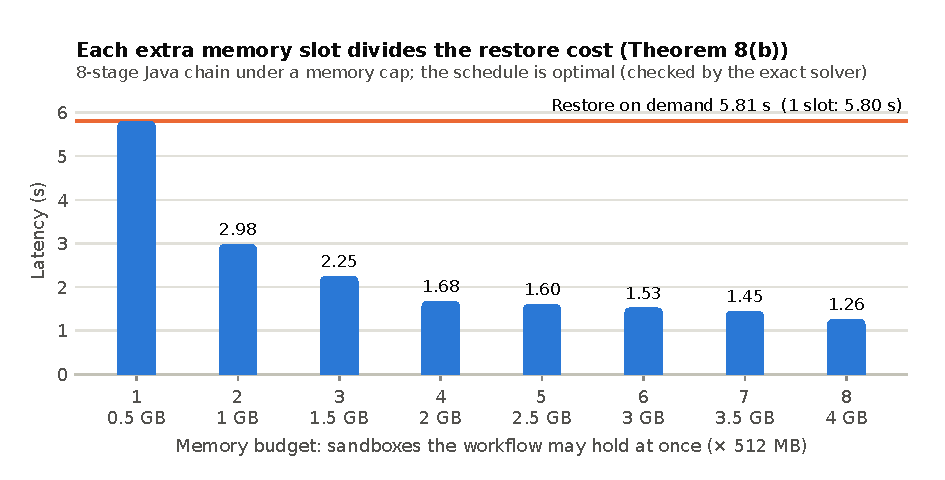
\includegraphics[width=0.8\textwidth]{fig3_memory_slots.pdf}
\caption{Latency of an eight-stage Java chain under look-ahead when at most $k$ sandboxes may
be alive at once (\cref{thm:memory}(b); $r = 650$\,ms, $w = 75$\,ms, $\delta = 2$\,ms). With
one slot it equals restoring on demand; each extra slot divides the restore cost.}
\label{fig:slots}
\end{figure}

% ------------------------------------------------------------------------------------------
\section{The problem behind the approach}
\label{sec:th-rcpsp}

This section shows that scheduling snapshot restores in a workflow is a classical
operations-research problem, identifies the results above as its tractable special cases, and
gives the exact method used for the rest.

\subsection{A sandbox is an activity, an edge is a time lag}

\begin{lemma}[No idle sandbox]
\label{lem:noidle}
% repo: Lemma A1 (ALGORITHM.md)
Some optimal schedule, under any memory budget, never lets a restored sandbox wait for its
input.
\end{lemma}

\begin{proof}
If $\tau_v + r_v < I_v$, move the trigger to $\tau'_v = I_v - r_v$. The stage still starts at
$I_v$, so no finish time changes, and it holds memory on $[\tau'_v, F_v) \subset [\tau_v, F_v)$,
so the memory in use never increases.
\end{proof}

So stage $v$ becomes one \emph{activity} of fixed length $p_v = r_v + w_v$ that holds $m_v$ for
its whole duration, and each edge $(u, v)$ becomes a start-to-start \emph{time lag}:
\begin{align}
  \tau_v &\ge \tau_u + p_u + \delta - r_v && \text{(look-ahead)} \label{eq:lag-ahead}\\
  \tau_v &\ge \tau_u + p_u + \delta       && \text{(on demand)}  \label{eq:lag-od}\\
  \tau_v &\ge 0 && \text{(the workflow arrives at $0$).} \notag
\end{align}
\emph{Look-ahead is exactly the shortening of every precedence lag by the successor's restore
time.} The lag can be negative: $v$'s restore may start before $u$ starts. Two consequences
follow. Every schedule without idle sandboxes holds the same memory$\cdot$time
$\sum_v m_v (r_v + w_v) = M_{\min}$; schedules differ only in \emph{when} they hold it. And the
earliest-start schedule of the lag network \eqref{eq:lag-ahead} is the JIT schedule of
\cref{thm:jit}, while that of \eqref{eq:lag-od} is the on-demand schedule. In the running
example the look-ahead lag is $727 - 650 = 77$\,ms instead of $727$\,ms.

\subsection{Which known problem}

\Cref{tab:rcpsp} maps the model to project scheduling. The problem is the \emph{multi-mode
resource-constrained project scheduling problem with generalised precedence relations},
MRCPSP/max \cite{dereyck1999}; with the modes fixed it is RCPSP/max
\cite{bartusch1988,neumann2003}. \Cref{tab:cases} lists its special cases and where each result
of this chapter sits.

\begin{table}[t]
\centering
\caption{The model as a project-scheduling problem.}
\label{tab:rcpsp}
\small
\begin{tabular}{@{}ll@{}}
\toprule
project scheduling & snapshot restores in a workflow \\
\midrule
project & one cold workflow invocation \\
activity & one stage's sandbox: restore and run, length $r_v + w_v$ \\
mode of an activity & cold start; snapshot of depth $K$, stored locally or remotely \\
generalised precedence (time lag) & edge: $\tau_v \ge \tau_u + p_u + \delta - r_v$ \\
renewable resource & memory (budget $C$); restore channels (\cref{cor:channels}) \\
non-renewable resource & snapshot storage, or money \\
makespan & workflow latency \\
\bottomrule
\end{tabular}
\end{table}

\begin{table}[t]
\centering
\caption{Special cases of the problem, their complexity, and the results of this chapter.}
\label{tab:cases}
\small
\begin{tabular}{@{}p{0.2\textwidth}p{0.25\textwidth}p{0.2\textwidth}p{0.27\textwidth}@{}}
\toprule
case & known problem & complexity & this chapter \\
\midrule
no budget, modes fixed & temporal scheduling: longest paths in the lag network &
  $O(|V| + |E|)$ & \cref{thm:lb,thm:jit} \\
+ random durations & stochastic PERT & per stage & \cref{thm:newsvendor} \\
+ branches & probabilistic networks & per branch & \cref{thm:branch} \\
choose modes, no budget & discrete time--cost trade-off & strongly NP-hard in general
  \cite{de1997}; SP reduction \cite{demeulemeester1996} & \cref{thm:joint}: $(\text{storage}, W,
  P)$ dynamic program \\
budget, equal chain & RCPSP/max, special structure & closed form & \cref{thm:memory}(b) \\
budget, general & RCPSP/max with one resource & strongly NP-hard (\cref{prop:nphard}) &
  exact branch and bound (\cref{alg:bb}); the guard as a heuristic \\
keep-alive between calls & online weighted caching & online & \cref{prop:keepalive}; GDSF
  \cite{cherkasova1998,faascache2021} \\
CPU for start-ups, no budget & flexible resource profiles \cite{naber2014}; preemptive deadline
  scheduling \cite{horn1974} & polynomial: max-flow and bisection & \cref{thm:cpu-flow}; one
  spare core: \cref{prop:cpu-onecore,prop:cpu-burst} \\
\bottomrule
\end{tabular}
\end{table}

\begin{proposition}[Hardness]
\label{prop:nphard}
Minimising the latency of one workflow under a memory budget is NP-hard in the strong sense.
\end{proposition}

\begin{proof}
With $r_v = 0$ (a stage that is already warm), $\delta = 0$ and $m_v = 1$ for all $v$, and
$C = k$, the lags \eqref{eq:lag-ahead} become finish-to-start precedences and the budget allows
$k$ activities at once: this is $P \mid \mathrm{prec} \mid C_{\max}$, which is strongly NP-hard
already with unit processing times \cite{ullman1975}.
\end{proof}

\subsection{The exact solver}

\Cref{alg:bb} is the standard branch and bound on minimal forbidden sets
\cite{bartusch1988}. A \emph{forbidden set} is a set of activities that run at the same instant
and together exceed the budget; it is minimal if removing any activity makes it fit.

\begin{algorithm}[t]
\caption{\textsc{Exact}: minimal latency of one workflow under a memory budget $C$.}
\label{alg:bb}
\begin{algorithmic}[1]
\State $\mathit{best} \gets$ latency of the memory guard (or of capped on demand, if lower)
\State \Call{Search}{$\emptyset$}
\Procedure{Search}{$\mathcal{E}$} \Comment{$\mathcal{E}$: added constraints ``$u$ ends before $v$ starts''}
  \State $\tau \gets$ earliest-start schedule of the lag network plus $\mathcal{E}$
    \Comment{longest paths}
  \If{$\tau$ does not exist (positive cycle) \textbf{or} $\mathrm{makespan}(\tau) \ge \mathit{best}$}
    \State \Return
  \EndIf
  \State $F \gets$ a minimal forbidden set of $\tau$
  \If{there is none}
    \State $\mathit{best} \gets \mathrm{makespan}(\tau)$; \Return
      \Comment{feasible: a better schedule}
  \EndIf
  \ForAll{ordered pairs $(u, v)$ of distinct activities in $F$}
    \State \Call{Search}{$\mathcal{E} \cup \{\tau_v \ge \tau_u + p_u\}$}
  \EndFor
\EndProcedure
\end{algorithmic}
\end{algorithm}

\begin{proposition}[Exactness]
\label{prop:bb}
\Cref{alg:bb} returns the minimal latency under the budget $C$.
\end{proposition}

\begin{proof}
Intervals on a line that overlap pairwise share a common point (the Helly property). So in any
schedule that respects the budget, some two activities of $F$ do not overlap: one ends before
the other starts, and the loop covers every such choice. The earliest-start schedule of each
branch is the pointwise earliest schedule meeting its constraints, so its makespan bounds every
schedule in the branch from below, and pruning at $\mathit{best}$ is safe.
\end{proof}

In pure Python on one core, \cref{alg:bb} solves random workflows of up to 8 stages in about
$1$\,ms at the median ($0.1$\,s at worst for chains, $1.3$\,s for general DAGs) and 10-stage DAGs
in $21$\,ms at the median, with a heavy tail ($12$\,s at the 95th percentile). Real workflows are
small: in Azure's workflows the median depth is 3 and the 95th percentile 8 \cite{orion2022}. The
platform runs the solver with a node budget and keeps the best schedule found, which is never
worse than the guard's, because the search starts from it.

\begin{figure}[t]
\centering
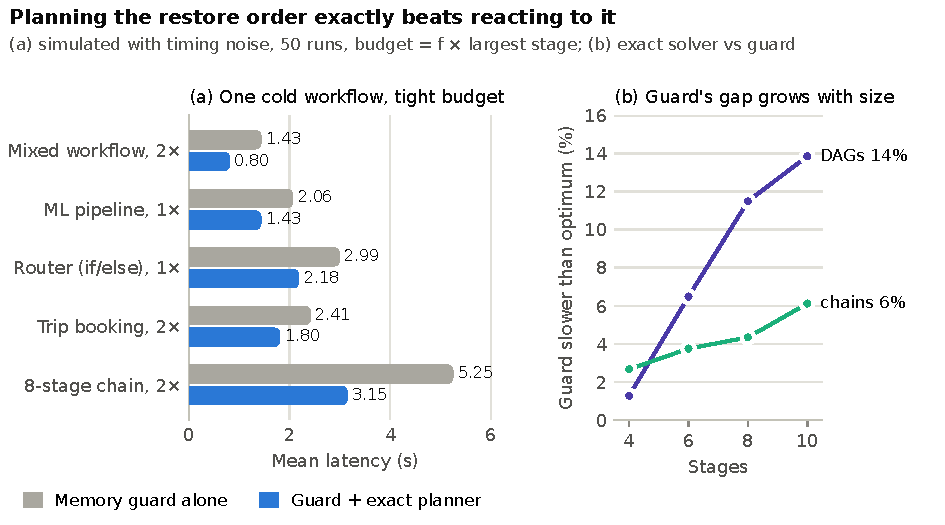
\includegraphics[width=\textwidth]{fig6_planner.pdf}
\caption{(a) One cold workflow under a tight memory budget, simulated with timing noise: the
memory guard alone against the guard executing an exact plan. (b) The guard's distance from
the optimum on random workflows, by size.}
\label{fig:planner}
\end{figure}

Against this optimum, the guard is optimal on $67$--$77\%$ of instances with 3--8 stages and
$3$--$5\%$ slower on average, but the gap grows with size (a mean of $14\%$ for 10-stage DAGs)
and reaches $87\%$ in the worst case (\cref{fig:planner}b). The guard reacts to whichever stage
is ready; the plan knows which stage is the long pole. In the smallest example we found, a
Python entry feeds a Java--Java chain and a machine-learning stage under a 1\,GB budget: the
guard gives the memory to the ML stage, whose input arrives first, and takes $1.93$\,s; the
optimum makes the ML stage wait, although its input is there, because it can finish behind the
chain, and takes $1.29$\,s.

\subsection{Restore contention as a second resource}

Restores that slow each other (\cref{cor:contention}) fit the same model as a second renewable
resource: $c$ restore channels, each restore holding one channel for $r_v$.

\begin{corollary}[Restore channels]
\label{cor:channels}
% repo: Corollary A3 (ALGORITHM.md)
On a chain of equal stages with $c$ restore channels and no memory budget, the schedule
$\tau_v = \max(\tau_{v-1} + w + \delta,\; \tau_{v-c} + r)$ is feasible, and on long chains each
stage costs $\max(w + \delta, r/c)$. It equals the exact solver's optimum on every instance
tested (check A3).
\end{corollary}

Each channel divides the restore cost, as each memory slot does in \cref{thm:memory}(b). For a
five-stage Java chain (on demand $3.63$\,s), $c = 1, 2, 4, 9$ give $3.33$, $2.02$, $1.38$ and
$1.03$\,s. A measured contention $\beta$ behaves roughly like $c \approx 1/\beta$ channels.

\subsection{The algorithm}

The platform runs four procedures. \Cref{alg:build} runs at deployment and reads no user data;
\cref{alg:plan,alg:run} run for each cold workflow arrival; keep-alive runs between calls.

\begin{algorithm}[t]
\caption{\textsc{Build} (per function, at each deployment).}
\label{alg:build}
\begin{algorithmic}[1]
\State profile with the developer's test requests at the serving CPU size: $A$, $B$, $r(K)$,
  $s(K)$, $m$
\State choose snapshot points: after start-up; for JIT runtimes also after warm-up, stopping
  when the JIT's compile counters flatten (\cref{prop:depth})
\State modes per stage: cold $\mid$ snapshot$(K)$ local $\mid$ snapshot$(K)$ remote
\State choose modes with the $(\text{storage}, W, P)$ dynamic program (\cref{thm:joint}); pick a
  point of the front by storage budget, price or latency target (\cref{cor:price})
\State checkpoint after reset hooks have re-seeded random state and removed secrets
\end{algorithmic}
\end{algorithm}

\begin{algorithm}[t]
\caption{\textsc{Plan} (per cold workflow arrival).}
\label{alg:plan}
\begin{algorithmic}[1]
\State set $r_v \gets 0$ for every stage that has an idle warm sandbox
\State keep the likely path: stages reached with probability at least $1/2$
\State $\tau \gets$ earliest start of the lag network \eqref{eq:lag-ahead}
  \Comment{the JIT schedule, \cref{thm:jit}}
\State $C_w \gets$ memory this workflow may use now (free, plus idle sandboxes it may evict)
\If{$\mathrm{peak}(\tau) \le C_w$} \Return $\tau$ \Comment{optimal}
\EndIf
\If{the platform is over budget, or was within the last minute} \Return $\tau$
\EndIf
\State $\tau' \gets$ \Call{Exact}{$G, C_w$} with a node budget \Comment{\cref{alg:bb}}
\If{$\mathrm{latency}(\tau') \ge$ the on-demand latency} \Return $\tau$
\EndIf
\State \Return $\tau'$
\end{algorithmic}
\end{algorithm}

\begin{algorithm}[t]
\caption{\textsc{Run} (event-driven, shared by all workflows on a machine).}
\label{alg:run}
\begin{algorithmic}[1]
\On{trigger $\tau_v$}
  \State restore $v$; if it does not fit, $v$ waits in a queue until memory frees
\EndOn
\On{input of $v$}
  \State start $v$ on its restored sandbox; a planned stage whose trigger is later waits for it
\EndOn
\On{deadline $\tau_v + r_v$ passed while $v$ waits}
  \State fall back to the guard of \cref{thm:memory}(c): a demand start that may preempt
    unclaimed look-ahead sandboxes
\EndOn
\On{any stage finishes}
  \State if the rest of a planned workflow now fits in the memory it can get, drop its plan and
    use JIT triggers
\EndOn
\end{algorithmic}
\end{algorithm}

Between calls, idle sandboxes are evicted per function by GreedyDual-Size-Frequency
\cite{cherkasova1998,faascache2021,cidre2025}: priority $=$ clock $+$ frequency $\times$ restore
cost $/$ memory. The simulator showed that each rule of \cref{alg:plan,alg:run} is needed: without
the likely-path rule, the queue, the re-planning, or the two rules that switch planning off,
the planner loses to the guard in some setting.

\paragraph{Keep-alive under look-ahead.} Keep-alive policies value a warm sandbox at its own
cold-start cost. For a cold arrival served by look-ahead that valuation is wrong:

\begin{proposition}[Keep-alive is a threshold decision per workflow]
\label{prop:keepalive}
% repo: Proposition 9 (ALGORITHM.md)
Let $\mathcal{W}$ be the set of stages with an idle warm sandbox when a workflow with one entry
arrives. Then
\begin{enumerate}[label=(\alph*)]
  \item its look-ahead latency is
        $L(\mathcal{W}) = \max\bigl(\ell(e),\; \max_{v \notin \mathcal{W}} (r_v + \ell(v))\bigr)$;
  \item the best $k$ stages to keep warm are the $k$ with the largest $r_v + \ell(v)$;
  \item on a chain of $d$ equal stages, keeping the first $j < d$ warm saves $\min(r, j(w +
        \delta))$, and keeping all $d$ warm saves $r$.
\end{enumerate}
\end{proposition}

\begin{proof}
(a) is \cref{thm:lb} with $r_v = 0$ for the warm stages. (b) By (a) the latency depends only on
the largest $r_v + \ell(v)$ left outside $\mathcal{W}$, so a top-$k$ set is best. (c)
$\ell(1) - \ell(j + 1) = j(w + \delta)$.
\end{proof}

On a five-stage Java chain, keeping only the entry warm saves $77$\,ms, not the $650$\,ms a
per-function policy assumes. Tested as an eviction policy on the Azure trace, however, evicting
whole workflows lost to per-function GDSF: most arrivals are hot, the entry gate then skips
look-ahead, and a missing stage costs its full restore, which is the per-function valuation. The
proposition therefore stays a statement about cold arrivals, and the platform uses GDSF.

% ------------------------------------------------------------------------------------------
\section{When to stop warming up}
\label{sec:th-depthwork}

Build-time warm-up needs a stopping rule that does not depend on what the requests contain.

\begin{proposition}[Depth is work, not requests]
\label{prop:depth}
% repo: Proposition 8
Under threshold tiered compilation without deoptimisation, method $\mu$ reaches tier $t$ after
a set $\mathcal{P}$ of warm-up requests if and only if $c_\mu(\mathcal{P}) \ge \theta_t$, where
$c_\mu(\mathcal{P}) = \sum_{x \in \mathcal{P}} n_\mu(x)$ counts its invocations. Hence
$\mathcal{P} \subseteq \mathcal{P}'$ implies that every method compiled after $\mathcal{P}$ is
compiled after $\mathcal{P}'$: adding requests never un-compiles. The number of requests is not
a sufficient statistic; the counters are.
\end{proposition}

\begin{proof}
The counters are additive over requests and thresholds are fixed, so $c_\mu$ is monotone in
$\mathcal{P}$. Two sets of equal size can differ in $c_\mu$ by the ratio of per-request work.
\end{proof}

Receiver-type pollution and deoptimisation can make a larger warm-up set compile slower code,
so the performance consequence is empirical. The rule: stop warming up when the JIT's
compile counter stops rising (in HotSpot, from \texttt{hsperfdata} or JFR). In our measurements
the compiled-method count at the snapshot rose monotonically with warm-up work.

% ------------------------------------------------------------------------------------------
\section{Planning CPU for start-ups}
\label{sec:th-cpu}
% repo: theory/CPU_PLAN_THEORY.md (results CP1-CP7)

So far every start-up had a fixed length: a restore took $r_v$. That length depends on the CPU
the sandbox gets. Starting a function is CPU work (restoring memory, loading classes, compiling
hot methods), and serverless functions get small CPU shares. In our measurements the same JVM
warm-up took $3.59$\,s at $0.25$\,vCPU and $0.86$\,s at $1$\,vCPU, for the same CPU time ($0.90$
and $0.86$\,CPU-seconds; \chapref{ch:model}{Chapter~3}). A server's spare CPU can therefore
shorten start-ups without costing CPU time. But it is limited, and a cold workflow starts several
sandboxes at once, so who gets it, and when, decides how fast the workflow starts. Cloud Run's
startup CPU boost gives every starting instance the same extra CPU \cite{cloudrunboost}; ORION
sizes each stage once, for its whole run \cite{orion2022}. This section makes the CPU of each
start-up a decision over time, planned from the workflow graph. The results of
\cref{sec:th-optimal} are its special case with no spare CPU.

\subsection{Model}

\begin{definition}[CPU plan]
\label{def:cpuplan}
% repo: CPU_PLAN_THEORY.md section 1
Each stage $v$ of a workflow (\cref{def:workflow}) has a \emph{start-up} of CPU work $U_v > 0$,
in CPU-seconds: a snapshot restore plus the first request's residual warm-up, or a cold boot plus
the full warm-up. The start-up can use at most $c_v > 0$ cores (its \emph{cap}), and it has a
\emph{private quota} $q_v \in [0, c_v]$ that no other start-up can use. It may begin at its
\emph{release} $a_v \ge 0$; under look-ahead $a_v = 0$. The server has \emph{spare CPU}
$\Pi(t) \ge 0$, piecewise constant: the CPU the running requests leave. A \emph{CPU plan} gives each
start-up a rate $x_v(t) = y_v(t) + z_v(t)$ for $t \ge a_v$, with a private part
$0 \le y_v(t) \le q_v$, a shared part $z_v(t) \ge 0$, $x_v(t) \le c_v$, and
$\sum_v z_v(t) \le \Pi(t)$. Start-up $v$ is \emph{ready} at the time $\rho_v$ at which
$\int_{a_v}^{\rho_v} x_v = U_v$. The schedule is that of \cref{def:schedule} with $\tau_v + r_v$
replaced by $\rho_v$: $S_v = \max(\rho_v, I_v)$ and $F_v = S_v + w_v$.
\end{definition}

The platform can enforce a plan: it sets each starting sandbox's CPU limit (cgroup
\texttt{cpu.max}) and lowers it to the function's normal share once the start-up is done. The
plan used by the simulator sets $q_v = 0$: a start-up is guaranteed nothing, so a start-up that
is not urgent cannot hold CPU that an urgent one needs. \Cref{tab:cpu-assumptions} lists the
assumptions.

\begin{table}[htbp]
\centering
\caption{Assumptions of the CPU plan.}
\label{tab:cpu-assumptions}
\small
\begin{tabular}{@{}p{0.2\textwidth}p{0.36\textwidth}p{0.36\textwidth}@{}}
\toprule
assumption & statement & status \\
\midrule
B1 linear speed-up & a start-up given rate $x \le c_v$ does its work $U_v$ in $U_v / x$ &
  measured for JVM warm-up from $0.25$ to $1$\,vCPU ($4.2\times$ faster at the same CPU time);
  an assumption for restores and cold starts, to be measured \\
B2 separate requests & running requests keep their CPU share; start-ups use only $\Pi(t)$ & the
  platform's choice (a CPU limit per sandbox) \\
B3 known work & $U_v$ and $w_v$ are profiled & as A2 and A3; under uncertainty use quantiles
  (\cref{thm:newsvendor}) \\
B4 look-ahead & a start-up may begin when its workflow arrives & as in \cref{sec:th-optimal} \\
\bottomrule
\end{tabular}
\end{table}

\subsection{Deadlines per start-up}

\begin{lemma}[Deadlines per start-up]
\label{lem:cpu-deadlines}
% repo: Lemma CP1
For every CPU plan the latency is $L = \max_{v \in V} \bigl(\rho_v + \ell(v)\bigr)$. Hence
$L \le \Lambda$ if and only if every start-up is ready by its \emph{deadline}
$D_v(\Lambda) := \Lambda - \ell(v)$.
\end{lemma}

\begin{proof}
As in the proof of \cref{thm:lb}(b), with $r_v$ replaced by $\rho_v$. By induction in
topological order, $F_v = \max_{u, P} \bigl(\rho_u + W(P)\bigr)$ over the ancestors $u$ of $v$
(including $v$) and the paths $P$ from $u$ to $v$: at the entry $F_e = \rho_e + w_e$ because
$I_e = 0 \le \rho_e$, and for $v \ne e$ the term $\rho_v + w_v$ covers $u = v$ while
$\max_{u \in \pred(v)} F_u + \delta + w_v$ extends every path into a predecessor by one edge. At
the sinks this is $\max_u \bigl(\rho_u + \ell(u)\bigr)$. The equivalence holds because $L$ is a
maximum of the terms $\rho_v + \ell(v)$.
\end{proof}

The lemma turns ``finish the workflow soon'' into ``every start-up meets its own deadline''. The
deadlines depend on the target $\Lambda$ only through a common shift, and the most urgent
start-ups are those with the longest remaining path $\ell(v)$.

\subsection{The exact plan}

\begin{theorem}[The exact CPU plan]
\label{thm:cpu-flow}
% repo: Theorem CP2
Fix a target $\Lambda$ and let $D_v = \Lambda - \ell(v)$. Cut the time axis at every release,
every deadline and every breakpoint of $\Pi$ into slices $I_1, I_2, \dots$, and let $\Pi_k$ be the
spare CPU on $I_k$. Build a network with a source, a sink, one node per start-up and one node per
slice, and the arcs
\begin{itemize}
  \item source $\to v$, capacity $U_v$;
  \item $v \to$ sink, capacity $q_v \max(0, D_v - a_v)$ (the private quota);
  \item $v \to k$ for every slice $I_k \subseteq [a_v, D_v]$, capacity $(c_v - q_v)\,|I_k|$;
  \item $k \to$ sink, capacity $\Pi_k\,|I_k|$.
\end{itemize}
Then a CPU plan with latency at most $\Lambda$ exists if and only if a maximum flow saturates
every source arc, and such a flow gives the plan. Feasibility is monotone in $\Lambda$, so
bisection on $\Lambda$ finds the optimal latency $L^*_\Pi$ to any precision.
\end{theorem}

\begin{proof}
By \cref{lem:cpu-deadlines}, latency at most $\Lambda$ means $\rho_v \le D_v$ for every $v$.
\begin{itemize}
  \item \emph{A flow gives a plan.} Let $g_v$ be the flow on $v$'s private arc and $f_{vk}$ on
        its arc to slice $k$. Run $v$ at private rate $g_v / (D_v - a_v) \le q_v$ over its window
        and at shared rate $f_{vk} / |I_k| \le c_v - q_v$ in slice $k$. The shared rates in a
        slice sum to at most $\Pi_k$, the total rate is at most $c_v$, and the work done by $D_v$ is
        $g_v + \sum_k f_{vk} = U_v$.
  \item \emph{A plan gives a flow.} Integrate the private part $y_v$ over the window and the
        shared part $z_v$ over each slice. Every capacity holds, and the flow out of $v$ is the
        work done by $D_v$, which is $U_v$.
  \item \emph{Monotonicity.} A larger $\Lambda$ moves every deadline later, so a plan for
        $\Lambda$ is a plan for every $\Lambda' > \Lambda$. \qedhere
\end{itemize}
\end{proof}

This is Horn's flow construction for preemptive scheduling with release times and deadlines
\cite{horn1974}, with a rate cap per job. In project-scheduling terms, the start-ups are
activities whose duration depends on how much of a resource they get: project scheduling with
flexible resource profiles \cite{naber2014}. The problems of \cref{sec:th-rcpsp} fix the
durations.

\begin{corollary}[A certificate]
\label{cor:cpu-cut}
% repo: Corollary CP2.1
No CPU plan reaches $\Lambda$ if and only if some set $T$ of start-ups has
\[
  \sum_{v \in T} U_v \;>\; \sum_{v \in T} q_v \max(0, D_v - a_v)
  + \int_0^\infty \min\Bigl(\Pi(t),\; \sum_{v \in T,\; a_v \le t < D_v} (c_v - q_v)\Bigr)\, dt .
\]
\end{corollary}

\begin{proof}
Max-flow/min-cut. A cut that keeps the start-ups of $T$ on the source side cuts the source arcs
of all others, the private arcs of $T$, and in each slice either the arcs from $T$ or the slice's
arc to the sink, whichever is smaller. Its capacity is therefore
$\sum_{v \notin T} U_v$ plus the right-hand side, and the flow saturates every source arc if and
only if no such cut has capacity below $\sum_v U_v$.
\end{proof}

Such a set $T$ proves that the target cannot be met; it is a lower bound that needs no search.

\begin{proposition}[The two extremes]
\label{prop:cpu-limits}
% repo: Proposition CP3
Let every $a_v = 0$.
\begin{enumerate}[label=(\alph*)]
  \item With no spare CPU ($\Pi \equiv 0$) and $q_v > 0$, the optimal latency is
        $\max_v (U_v / q_v + \ell(v))$: the $L^*$ of \cref{thm:lb} with $r_v = U_v / q_v$.
  \item With spare CPU at least $\sum_v (c_v - q_v)$ at all times, it is
        $L_{\mathrm{ideal}} = \max_v (U_v / c_v + \ell(v))$.
  \item The optimal latency is non-increasing in $\Pi$.
\end{enumerate}
\end{proposition}

\begin{proof}
(a) Without shared CPU, start-up $v$ is ready no earlier than $U_v / q_v$, and running every
start-up at its quota from time $0$ attains that; \cref{lem:cpu-deadlines} gives the maximum.
(b) Every start-up can run at its cap from time $0$, and none can be ready before $U_v / c_v$.
(c) A plan for $\Pi$ is a plan for any $\Pi' \ge \Pi$.
\end{proof}

So the CPU plan interpolates between the fixed-CPU look-ahead of \cref{thm:lb} ($\Pi = 0$) and the
ideal, in which every start-up runs at full speed.

\subsection{One spare core}

\begin{proposition}[One spare core]
\label{prop:cpu-onecore}
% repo: Proposition CP4
Let $q_v = 0$, $a_v = 0$ and $\Pi(t) \le c_v$ for all $v$ and $t$: the spare CPU never exceeds what
one start-up can use.
\begin{enumerate}[label=(\alph*)]
  \item Running the start-ups one at a time, earliest deadline first (longest $\ell(v)$ first),
        each at rate $\Pi(t)$, is optimal.
  \item On a chain of $d$ stages with constant $\Pi$, the optimum $L^*_\Pi$ and restoring on demand
        with the same boost, $L_{\mathrm{od},\Pi} = \sum_v (U_v / \Pi + w_v) + (d - 1)\delta$,
        satisfy
        \[
          0 \le L_{\mathrm{od},\Pi} - L^*_\Pi \le \sum_{v < d} w_v + (d - 1)\,\delta ,
        \]
        with equality when the chain is CPU-bound, that is when
        $L^*_\Pi = \sum_v U_v / \Pi + w_d$.
\end{enumerate}
\end{proposition}

\begin{proof}
(a) Number the start-ups so that $\ell(v_1) \ge \ell(v_2) \ge \dots$ and let
$\bar\Pi(t) = \int_0^t \Pi$. Earliest deadline first makes $v_k$ ready at $\rho_k$, the first time $\bar\Pi$
reaches $U_{v_1} + \dots + U_{v_k}$. In any plan the rates sum to at most $\Pi(t)$, so the first $k$
start-ups cannot all be ready before $\rho_k$: some $v_i$ with $i \le k$ is ready at
$\rho'_{v_i} \ge \rho_k$, and $\ell(v_i) \ge \ell(v_k)$. By \cref{lem:cpu-deadlines} that plan's
latency is at least $\rho_k + \ell(v_k)$ for every $k$, which is the latency of earliest
deadline first. This is Jackson's rule \cite{jackson1955}.

(b) Restoring on demand is a plan, so $L^*_\Pi \le L_{\mathrm{od},\Pi}$. In any plan the last
start-up to be ready, say $v$, is ready no earlier than $\sum_u U_u / \Pi$, and $\ell(v) \ge w_d$ on
a chain, so $L^*_\Pi \ge \sum_u U_u / \Pi + w_d$ by \cref{lem:cpu-deadlines}. Subtracting gives the
bound, with equality exactly when this lower bound is attained.
\end{proof}

With about one core to spare, look-ahead can only overlap start-ups with the stages' own run
times, $\sum (w + \delta)$: about $0.1$\,s on a three-stage Java chain at $0.25$\,vCPU. This is
why, in the simulator, the CPU plan only ties with the startup boost on one spare core.
The parallelism of look-ahead needs more than one spare core.

\subsection{Branches}

\begin{proposition}[Leftover speculation]
\label{prop:cpu-spec}
% repo: Proposition CP5
If the start-ups of stages that may not run (behind an if/else not yet decided) get only the CPU
that the certain start-ups' plan leaves, every certain start-up is ready exactly when it would be
without them.
\end{proposition}

\begin{proof}
The certain start-ups' rates are computed without the speculative ones, which use only what is
left at each instant.
\end{proof}

\begin{proposition}[The cost of a wrong guess]
\label{prop:cpu-wrong}
% repo: Proposition CP6
Under the conditions of \cref{prop:cpu-onecore} with constant $\Pi$, let a speculative start-up $s$
be served as if certain, ahead of some certain start-ups in earliest-deadline order, and let its
branch not be taken. Then every certain start-up after it is ready $U_s / \Pi$ later, and a
CPU-bound chain finishes exactly $U_s / \Pi$ later.
\end{proposition}

\begin{proof}
One start-up runs at a time at rate $\Pi$, so inserting $U_s$ of work before them shifts each later
ready time by $U_s / \Pi$. When the chain is CPU-bound its latency is the last ready time plus
$w_d$.
\end{proof}

So serving a branch reached with probability $p$ as certain pays in expectation only if
$p\, G \ge (1 - p)\, U_s / \Pi$, where $G$ is what its early start saves when the branch is taken.
By \cref{prop:cpu-onecore}(b), $G$ is at most the overlap with the run times, $\sum (w + \delta)$
along its path. With the measured Java values on one spare core ($U_s / \Pi \approx 0.7$\,s,
$G \approx 0.05$\,s) this needs $p \ge 0.93$. The rule has the form of \cref{thm:branch}
(speculate if and only if $p \ge \kappa$), with CPU time as the cost. Hence the online rule
below: with at most one spare core only stages certain to run are served as certain, and with
more the likely path is, as in \cref{alg:plan}.

\subsection{Bursts}

\begin{proposition}[Bursts on one spare core]
\label{prop:cpu-burst}
% repo: Proposition CP7
Workflows $w$ arrive at times $t_w$, with $q_v = 0$ and $\Pi(t) \le c_v$. Give each start-up $v$ of
workflow $w$ the release $t_w$ and the deadline $t_w + \Lambda_w - \ell(v)$, where $\Lambda_w$ is
the ideal latency of $w$ (\cref{prop:cpu-limits}(b)). Then preemptive earliest deadline first
minimises the largest delay of any workflow over its ideal, $\max_w (L_w - \Lambda_w)$.
\end{proposition}

\begin{proof}
By \cref{lem:cpu-deadlines} applied to each workflow,
$L_w - \Lambda_w = \max_{v \in w} (\rho_v - D_v)$, so $\max_w (L_w - \Lambda_w)$ is the largest
lateness over all start-ups. Each start-up can absorb all the spare CPU, so in the time scale
$\bar\Pi(t) = \int_0^t \Pi$ this is preemptive scheduling on one machine with release times, minimising
the largest lateness, for which preemptive earliest deadline first is optimal \cite{horn1974}.
\end{proof}

With more than one spare core, greedy earliest deadline first is not optimal (the
multiprocessor case \cite{dhall1978}). The exact plan then comes from \cref{thm:cpu-flow}, with
one common shift added to all deadlines and minimised by bisection.

\subsection{Just in time}

A start-up that begins when its workflow arrives holds its sandbox's memory from then until its
stage finishes, and with little CPU it holds it for long: in the simulator the plan as described
so far held up to $11\times$ the memory$\cdot$time of restoring on demand with an equal
startup boost. For fixed restore
times, \cref{thm:jit} solved this by starting each restore just in time. Here when a start-up
begins interacts with the CPU the others get.

\begin{proposition}[Just in time]
\label{prop:cpu-jit}
% repo: Proposition CP8
\begin{enumerate}[label=(\alph*)]
  \item Let the targets $D_v$ be feasible (\cref{thm:cpu-flow}). Taking the start-ups latest
        target first, move each one's release as late as the network stays feasible. Then the
        final releases are feasible, and no single release can move later.
  \item Let a sandbox hold memory $m_v$ from the first time its start-up gets CPU, $\sigma_v$,
        until its stage finishes. Under the conditions of \cref{prop:cpu-onecore}, with constant
        $\Pi$, every plan holds at least $\sum_v m_v (U_v / \Pi + w_v)$, the memory$\cdot$time
        of restoring on demand with the same boost. On a chain with
        $U_{v+1} / \Pi \ge w_v + \delta$ for every $v$, running the start-ups one at a time,
        each holding memory only from its first CPU, attains this minimum and the optimal
        latency $\sum_v U_v / \Pi + w_d$ together.
\end{enumerate}
\end{proposition}

\begin{proof}
(a) Feasibility is monotone in each release: a later release shrinks a window, and a plan for
the smaller window is a plan for the larger one. The moves accept only feasible releases, so
feasibility holds throughout. When $v$ was moved, the start-ups moved after it had releases no
later than their final ones; moving them later only removes plans, so $v$ still cannot move
later.

(b) A start-up gets at most $\Pi$ at any instant, so it is ready no earlier than
$\sigma_v + U_v / \Pi$, and $F_v \ge \rho_v + w_v$. One at a time, start-up $v$ runs from
$\sum_{u < v} U_u / \Pi$ to $\rho_v = \sum_{u \le v} U_u / \Pi$. If stage $v - 1$ started at
$\rho_{v-1}$, the input of $v$ arrives at $\rho_{v-1} + w_{v-1} + \delta \le \rho_v$, so stage $v$
starts at $\rho_v$ and $F_v - \sigma_v = U_v / \Pi + w_v$; by induction this holds for every
stage. The latency is $F_d = \sum_v U_v / \Pi + w_d$, the lower bound in the proof of
\cref{prop:cpu-onecore}(b).
\end{proof}

Part (b) is \cref{thm:jit} for the CPU plan on one spare core: again there is no trade-off
between latency and memory. With more spare CPU, (a) guarantees that holding start-ups back
gives up no reachable target; how much memory it saves is measured. The platform computes the
latest starts once, when a workflow arrives, on the stages likely to run, and triggers each
start-up a margin before its latest start; until then the start-up holds no memory and no CPU.
A CPU-bound workflow (its smallest lateness above the all-at-cap one) is the exception: there
idle CPU is lost time, so the next start-up runs rather than leave the CPU idle. Stages that may
not run are not held back, since they get only leftover CPU anyway (\cref{prop:cpu-spec}), and a
branch not taken cancels its start-ups. In the simulator this keeps the plan's latency (from
$8\%$ faster to $1.3\%$ slower) and cuts its memory$\cdot$time for one workflow by $49$--$88\%$ on
one spare core, where it then equals restoring on demand, by up to $73\%$ on two and $33\%$ on
four, and by $76$--$82\%$ in a burst of sixteen workflows.

\subsection{The online rule}

The exact plan needs the whole future. The platform runs a rule that is recomputed at every
event (\cref{alg:boost}).

\begin{algorithm}[t]
\caption{\textsc{Boost} (event-driven, per machine): CPU for start-ups.}
\label{alg:boost}
\begin{algorithmic}[1]
\On{a workflow arrives}
  \State latest start of each look-ahead start-up, less a margin \Comment{\cref{prop:cpu-jit}}
\EndOn
\On{a start-up or a request begins or ends, or a latest start passes}
  \State requests run at their quota; $\Pi \gets$ the machine's CPU that they leave
  \State give each start-up the deadline $t_w + \Lambda_w - \ell(v)$
    \Comment{\cref{lem:cpu-deadlines}}
  \State certain $\gets$ $p = 1$ if $\Pi \le$ one cap, else $p \ge 1/2$
    \Comment{\cref{prop:cpu-wrong}}
  \State hold back certain start-ups before their latest start, unless CPU-bound
    \Comment{\cref{prop:cpu-jit}}
  \If{one workflow and $\Pi >$ one cap}
    \State constant rates that minimise their largest lateness; share the rest equally
  \Else
    \State earliest deadline first, each up to its cap
      \Comment{\cref{prop:cpu-onecore,prop:cpu-burst}}
  \EndIf
  \State the other start-ups share what is left \Comment{\cref{prop:cpu-spec}}
  \State set each starting sandbox's CPU limit to its rate; it takes its memory now
\EndOn
\On{a branch is decided}
  \State cancel the start-ups of the branches not taken
\EndOn
\end{algorithmic}
\end{algorithm}

For one workflow the rule chooses, by bisection on the lateness, the constant rates that
minimise the largest lateness of its start-ups; they are optimal among plans whose rates stay
constant from now on. The exact plan can do better by giving CPU to the urgent start-ups first;
on our test workflows in a fluid model the rule is within $0$--$9\%$ of it, while an equal split,
the startup boost's rule, is up to $1.39\times$ slower. For several workflows the rule is
earliest deadline first: optimal for the largest delay on one spare core
(\cref{prop:cpu-burst}), and chosen by simulation beyond that. Each certain start-up is held
back to its latest start (\cref{prop:cpu-jit}). Not proved, and not claimed: a competitive ratio
for the online rule, the burst rule beyond one spare core, how much memory holding start-ups
back saves with more than one spare core, and anything about real speed-up curves (B1).

% ------------------------------------------------------------------------------------------
\section{Verification}
\label{sec:th-verification}

Each result of this chapter was checked by an independent computation in a verification program
(\texttt{theory/verify\_dag.py}, standard-library Python). Each check compares the result with a
computation that does not use it: exhaustive search, brute force over all options, an event-level
simulation, or Monte Carlo sampling. Each check is paired with a \emph{control}: a variant designed
to fail, which passes only if the check detects the violation. A check that cannot fail proves
nothing. The program runs 97 checks, 19 of them controls, and all pass.
\Cref{tab:checks,tab:checks-cpu} list the main ones.

\begin{table}[t]
\centering
\caption{Main checks in \texttt{theory/verify\_dag.py}. ``Control'' is the variant that must
fail.}
\label{tab:checks}
\small
\begin{tabular}{@{}p{0.18\textwidth}p{0.07\textwidth}p{0.4\textwidth}p{0.27\textwidth}@{}}
\toprule
result & check & what is compared & control \\
\midrule
\cref{thm:lb} & T1 & eager $= L^*$, on demand $= \ell'(e)$ on 2000 random DAGs; 150{,}000
  random policies never below $L^*$ & triggers before the arrival ($\tau < 0$) do beat $L^*$ \\
\cref{cor:chain} & C1.1 & closed forms, monotone speed-up and its bound, 384 parameter sets & \\
\cref{cor:contention} & C1.2 & the saving bound, analytically and in the simulator's contention
  model & \\
\cref{cor:random} & C1.3 & 18{,}006 Monte-Carlo instances & comparing with the deterministic
  bound fails \\
\cref{thm:jit} & T2 & 2000 DAGs; 30{,}000 random policies never below $M_{\min}$; the simulator's
  JIT reproduces $L^*$ and $M_{\min}$ & eager holds strictly more \\
\cref{thm:newsvendor} & T3 & the $\kappa$-quantile vs the numerical optimum, 3 distributions
  $\times$ 4 price ratios & the quantile $a/(a+b)$ costs more \\
\cref{thm:branch} & T4 & exact expected costs, 228 cases & \\
\cref{lem:gate} & L5 & gated $=$ ungated in the simulator, sequential calls & overlapping calls
  and an if/else workflow differ \\
\cref{thm:keepalive} & T6 & renewal Monte Carlo & \\
\cref{thm:joint} & T7 & composition rules vs the expanded DAG (2000 SP workflows); the dynamic
  program vs brute force (600) & a one-number state is wrong on 63/600 \\
\cref{cor:hidden,cor:tail} & T7 & 600 instances each & shortest tails first is worse \\
\cref{cor:price} & C7.3 & front vs brute force; lower hull; $\lambda e^{-\lambda T}$ & counting
  every call as cold ranks wrongly \\
\cref{thm:memory} & T8 & peak (2000 chains); recurrence vs slot simulation (1500); the guard
  (1500) & without preemption the guard deadlocks (582/1500) \\
\cref{lem:noidle}, \cref{prop:bb} & A1, A2 & lag network $=$ JIT and on demand (1000 DAGs);
  branch and bound vs brute force over all integer triggers (200) & \\
\cref{thm:memory}(b) optimal, \cref{cor:channels} & A3 & exact solver vs the closed forms (200 chains
  each) & \\
the guard's gap (\cref{sec:th-rcpsp}) & A4 & the exact optimum is never above the guard; gap
  statistics over 3000 capped instances & the guard is not optimal everywhere (838/3000) \\
\cref{alg:plan,alg:run} & A5, A6 & the guard executing the plan reaches the optimum with no
  preemption (800); the simulator's planner $=$ the exact solver & \\
\cref{prop:keepalive} & P9 & brute force over all $k$-sets & the per-function valuation
  overstates the saving for 99\% of stages \\
\bottomrule
\end{tabular}
\end{table}

\begin{table}[t]
\centering
\caption{Checks of the CPU plan (\cref{sec:th-cpu}) in \texttt{theory/verify\_dag.py}.}
\label{tab:checks-cpu}
\small
\begin{tabular}{@{}p{0.18\textwidth}p{0.07\textwidth}p{0.4\textwidth}p{0.27\textwidth}@{}}
\toprule
result & check & what is compared & control \\
\midrule
\cref{lem:cpu-deadlines} & CP1 & the latency formula and the deadlines, 2000 DAGs with random
  ready times & \\
\cref{thm:cpu-flow,cor:cpu-cut} & CP2 & max-flow vs the exhaustive subset condition (3000
  instances, with and without private quotas); the plan meets every deadline and a smaller target
  is infeasible (500 DAGs) & ignoring the caps changes the answer (172/500); an equal split is
  worse (398/500) \\
\cref{prop:cpu-limits} & CP3 & no and unlimited spare CPU, 500 DAGs each & \\
\cref{prop:cpu-onecore} & CP4 & earliest deadline first $=$ the exact plan (500 DAGs); the chain
  bound (250 chains) & one start-up at a time is worse with more than one spare core (443/500) \\
\cref{prop:cpu-spec,prop:cpu-wrong} & CP5, CP6 & 500 CPU-bound chains each & \\
\cref{prop:cpu-burst} & CP7 & earliest deadline first $=$ the exact smallest largest lateness
  (250 bursts) & greedy earliest deadline first is not optimal beyond one spare core (171/500) \\
\cref{prop:cpu-jit} & CP8 & latest starts stay feasible and none can move later (500 instances);
  one at a time holds the least memory at the optimal latency (250 chains) & an equal split from
  the arrival holds more memory (250/250) \\
\bottomrule
\end{tabular}
\end{table}

\Cref{tab:status} states the status of each kind of claim. What cannot be proved, and is not
claimed, are the absolute restore times and the contention $\beta$: they are properties of the
hardware, measured in \chapref{ch:evaluation}{Chapter~6}.

\begin{table}[t]
\centering
\caption{What is proved, what is verified, and what must be measured.}
\label{tab:status}
\small
\begin{tabular}{@{}p{0.55\textwidth}p{0.38\textwidth}@{}}
\toprule
claim & status \\
\midrule
look-ahead is latency-optimal; JIT is also memory-minimal; trigger and speculation rules &
  proved; verified on random DAGs and against the simulator \\
joint depth and timing on SP workflows; exact dynamic program; hidden cold starts &
  proved; verified against brute force \\
peak memory, $k$ slots, the guard's safety & proved \\
optimality of the $k$-slot and channel schedules & verified by the exact solver \\
the capped problem is RCPSP/max; exactness of the branch and bound & proved; verified against
  brute force \\
the guard's distance from the optimum; the planner under noise and load & measured on random
  DAGs; simulated \\
A2: restores run in parallel ($\beta$ small) & assumption, to be measured \\
A3: residual warm-up after a restore & assumption, to be measured \\
deadlines per start-up; the exact CPU plan; the fixed-CPU and ideal extremes; one spare core;
  speculation; bursts on one spare core; just in time & proved; verified against exhaustive
  enumeration and the exact plan \\
the online CPU rule's distance from the exact plan; the burst rule beyond one spare core; the
  memory just in time saves with more spare CPU & measured in a fluid model; chosen by
  simulation; simulated \\
B1: start-ups speed up linearly with CPU up to one core & measured for JVM warm-up; assumption
  for restores and cold starts, to be measured \\
no user data in any snapshot & by construction \\
\bottomrule
\end{tabular}
\end{table}

% ------------------------------------------------------------------------------------------
\section{Summary}
\label{sec:th-summary}

Restoring every stage of a cold workflow just in time, $\tau_v = S^*_v - r_v$, reaches the lowest
latency any policy can reach and holds the least memory$\cdot$time; on a chain it turns $d$
restores into one. Under uncertainty the trigger is a quantile, and branches are restored ahead
when their probability exceeds the same price ratio. Which stages deserve a snapshot, and how
deep, is decided exactly by a dynamic program with two numbers per sub-workflow; under
look-ahead, a stage's position in the workflow decides its value. Look-ahead raises the memory
peak, and under a budget each extra sandbox divides the restore cost.

The problem as a whole is resource-constrained project scheduling with time lags. The problem
class, the branch and bound and the list-scheduling heuristic are textbook operations research.
What this thesis contributes is the modelling (\cref{lem:noidle} turns a workflow of snapshot
restores into that problem), the special cases solved exactly and proved
(\cref{thm:lb,thm:jit,thm:newsvendor,thm:branch,thm:joint,thm:memory}), the $(W, P)$ state of the
dynamic program, the keep-alive analysis, and the measurements that calibrate the model.
Timing provisioning along the workflow graph is Xanadu's idea \cite{xanadu2020}; this thesis
applies it to snapshots, whose restore is short enough to hide, and proves what is optimal.

A start-up is CPU work, and its length depends on the CPU it gets. Planning the server's spare CPU
per start-up gives each start-up a deadline from the workflow graph (\cref{lem:cpu-deadlines}),
and the best plan is a maximum flow (\cref{thm:cpu-flow}). The fixed-CPU look-ahead of
\cref{thm:lb} is its case with no spare CPU. With about one spare core, earliest deadline first is
optimal, and look-ahead gains only the stages' own run times over starting on demand with the
same CPU (\cref{prop:cpu-onecore}); the planning pays where several start-ups compete for more
than one spare core. Held back to its latest start, a start-up gives up no reachable target, and
on one spare core the plan then also holds the least memory$\cdot$time (\cref{prop:cpu-jit}).

\bibliographystyle{plain}
\bibliography{theory}
\end{document}
